\documentclass{article}

\usepackage{arxiv}

\usepackage[utf8]{inputenc} % allow utf-8 input
\usepackage[T1]{fontenc}    % use 8-bit T1 fonts
\usepackage{hyperref}       % hyperlinks
\usepackage{url}            % simple URL typesetting
\usepackage{booktabs}       % professional-quality tables
\usepackage{amsfonts}       % blackboard math symbols
\usepackage{nicefrac}       % compact symbols for 1/2, etc.
\usepackage{microtype}      % microtypography
\usepackage{lipsum}
\usepackage{graphicx}
\graphicspath{ {./images/} }

\title{Master Thesis \\ \vspace{0.5cm}
    \small{Development and verification of MHD implementation of SPH-EXA}}

\author{
    Nicolas Müller \\
    D-MATH\\
    ETH Zürich\\
    \texttt{nicolmueller@ethz.ch} \\
}

\begin{document}
\maketitle
\begin{abstract}
This document for now serves as a dump for equations, plots and references and will later be turned into a proper report. \\ \\
Code \href{https://github.com/MuellerNico/sphexa/commits/develop/}{\textbf{GitHub fork}} \\
Progress write-up: \href{https://docs.google.com/document/d/1CMsmUqyYXGIk8lybewA6jtJdwgMwquEbrGCqE1sCMbo/edit?usp=sharing}{\textbf{Google docs}}
\end{abstract}

% keywords can be removed
%\keywords{First keyword \and Second keyword \and More}


\section{Background (copy of project description)}
The Smoothed Particles Hydrodynamics (SPH) is a particle-based, mesh-free, Lagrangian method used to simulate multidimensional fluids with arbitrary geometries, most commonly employed in astrophysics, cosmology, and computational fluid-dynamics.\cite{Rosswog2009} It was first developed by Gingold and Monaghan\cite{SPH-original} and Lucy\cite{SPH-original-2} in 1977. It is expected that these computationally demanding numerical simulations will significantly benefit from the up-and-coming Exascale computing infrastructures.

SPH-EXA is a \texttt{C++20} simulation code developed by the University of Basel for performing SPH simulations parallelized with \texttt{MPI}, \texttt{OpenMP}, \texttt{CUDA}, and \texttt{HIP} with the aim to enable said simulations to run on these Exascale systems.

A major goal in the SPH-EXA roadmap is to incorporate magnetic-field computations, as they are important in a wide array of different astrophysical systems\cite{WissingShen2020} and will increase the range of problems that can be simulated. For this, a magnetohydrodynamics (MHD) version of SPH-EXA is being developed together with a suite of relevant test cases, tackling problems where current resolution is the limiting factor. 

\subsection{Scope and Goals}
In this Master thesis project we seek to 

\begin{enumerate}
    \item continue the work on the development of the MHD version of SPH-EXA,
    \item improve on current test cases and develop additional test cases,
    \item study the possibility of using a slope-limited reconstruction method for the artificial resistivity instead of a heuristic switch,
    \item explore the scalability of the MHD implementation,
    \item and use the in-situ visualization infrastructure of SPH-EXA for generating plots at scale.
\end{enumerate}

\subsection{Sources}
Just listing them quickly to test bibtex
\begin{enumerate}
    \item SPH Introduction \cite{Rosswog2009}
    \item SPH-EXA release paper \cite{sphexa}
    \item SPH-EXA equations with new Volume Elements \cite{GarciaSenz2022}
    \item AV switches \cite{GarciaSenzCabezon2026}
    \item Wissing MHD reference \cite{WissingShen2020}
    \item MAGMA: Older MHD reference \cite{RosswogPrice2007}
    \item MHD switches \cite{TriccoPrice2013}
    \item Price conductivity formulations \& discontinuities in general \cite{Price2008}
    \item Gasoline2, conductivity choices \cite{Wadsley2017}
    \item Phantom \cite{Price2018}
    \item SPH-EXA turbulence paper \cite{Cabezon2026turb}
\end{enumerate}
\section{Introduction}

Smoothed-particle hydrodynamics (SPH) is a particle-based Lagrangian method used to simulate multidimensional fluids, most commonly employed in astrophysics, cosmology and computational fluid-dynamics. First developed by Gingold and Monaghan\cite{GingoldMonaghan1977} and Lucy\cite{Lucy1977} in 1977, it can outshine traditional grid-based Eulerian codes in some key areas such as its natural conservation properties \cite{Rosswog2009}, the handling of free surfaces and fluid interfaces \cite{He2024}, adaptive resolution \cite{Price2010} and it integrates well with fast gravity solvers for self-gravitating systems, which is particularly useful in astrophysical simulations. 

SPH-EXA is a high-performance \texttt{C++} code developed by the University of Basel for performing such SPH simulations on Exascale computing systems \cite{Cavelan2020}. It is parallelized with \texttt{MPI}, \texttt{OpenMP}, \texttt{CUDA}, and \texttt{HIP} to enable calculations with billions of particles running on thousands of hybrid CPU-GPU nodes in parallel. 

In most, if not all astrophysical problems, the influence of magnetic fields on plasma behavior is crucial in accurately describing them.\todo{concrete example} Therefore, many modern codes include a magnetohydrodynamic (MHD) extension for SPH (SPMHD). The primary goal of this project is to present a working and properly scaling implementation of SPMHD in SPH-EXA. The scalability of SPH-EXA will hopefully allow future simulations of large-scale MHD problems, which were previously limited by resolution constraints. 

In the following chapters we first briefly touch on the fundamentals of the SPH discretizations and how they are implemented in SPH-EXA using an integral approach to derivation. This will provide the necessary basis and context to then introduce the newly added magnetic field calculations. We base our implementation on other state-of-the-art SPMHD codes, namely \textsc{Phantom} \cite{Price2018} and the MHD extension to \textsc{Gasoline2} \cite{Wadsley2017, WissingShen2020}. 

We will give special focus to the treatment of discontinuities through artificial resistivity. Different approaches that emerged throughout the years are discussed. Then, we present a novel approach to limit unwanted dissipation, using slope-limited linear reconstruction of the local magnetic field, based on the same method recently proposed for artificial viscosity in \cite{GarciaSenzCabezon2026}. 

We then conduct a series of numerical tests to verify that our implementation produces results comparable to other SPMHD codes. There we also study the impact of different AR schemes, comparing our new design to a baseline implementation based on \cite{WissingShen2020}. As a final test we simulate subsonic magnetic turbulence at $N=1600^3$ particles as a proof of concept that SPH-EXA is now properly equipped to take on real astrophysical MHD problems beyond standardized tests. 

In chapter \ref{sec:performance} we study performance in a strong and weak scaling analysis, ensuring that the MHD extension scales together with the hydrodynamic parts of SPH-EXA. We also quantify the exact overhead on runtime in a per-kernel analysis. 

Finally, the key findings are discussed and next steps are outlined. 

Throughout this thesis paper we will heavily rely on Wissing \& Shen (2020) \cite{WissingShen2020} and Price et al. (2018) \cite{Price2018} as our primary reference both regarding the numerical method and as direct comparison for the tests in our verification suite. 

It is important at this point to properly credit Helena Schmidt (University of Basel), who wrote considerable parts of the current MHD module in SPH-EXA. The bulk work of this thesis project could therefore be focused on updating, validating, extending, optimizing and formalizing this implementation, rather than building it from scratch. 
\section{Theory}
\subsection{SPH Theory}
\subsection{MHD Theory}
% Magnetic Pressue
% \begin{equation}
% P_\text{mag} = \frac{|B|^2}{2\mu_0} = \frac{B_x^2 + B_y^2 + B_z^2}{2\mu_0}    
% \end{equation}

% MHD Stress Tensor
% \begin{equation}
% S^{ij} = -\delta^{ij}\left(P + \frac{B^2}{2}\right) + B^i B^j  
% \end{equation}

Induction Equation
\begin{equation}
    \frac{d\mathbf{B}}{dt} = (\mathbf{B}\cdot\nabla)\mathbf{v} - \mathbf{B}(\nabla\cdot\mathbf{v})
\end{equation}

Normalized divergence error
\begin{equation}
\epsilon_{\mathrm{divB}} = \frac{h\,|\nabla\cdot\mathbf{B}|}{|\mathbf{B}|}
\end{equation}

Divergence cleaning
\begin{equation}
    \left(\frac{d\mathbf{B}}{dt}\right)_\psi = -\nabla\psi \\ 
\end{equation}

\begin{equation}
\frac{d}{dt}\!\left(\frac{\psi}{c_h}\right) = -c_h\,\nabla\cdot\mathbf{B} 
  - \frac{1}{\tau}\frac{\psi}{c_h} - \frac{1}{2}\psi(\nabla\cdot\mathbf{v})
\end{equation}

\subsection{Artificial Resistivity}
Discontinuities
\subsubsection{Classic}
\subsubsection{Switches}
Tricco \& Price switch
\begin{equation}
\alpha_{B,a} = \frac{h_a\,|\nabla\mathbf{B}_a|}{|\mathbf{B}_a|}, \qquad \alpha_B \in [0,\,1]
\end{equation}
\subsubsection{SLR}


\section{Implementation}
Numerics, kernels, discrezation, software stuff
\section{Numerical Tests}
\label{sec:numerical_tests}
In this chapter we present the results produced by SPH-EXA on a suite of standard MHD tests. With the first seven test cases we verify that our implementation produces results comparable to the reference codes \cite{WissingShen2020, Price2018}. We quantify accuracy, observe the mean divergence error $\langle \varepsilon_{\text{divB}}\rangle$ \eqref{eq:divb_error} and inspect magnetic energy loss through resistive heating. In a final test we apply a magnetic field to subsonic turbulence in a high-resolution simulation.

The test setups closely follow those also used in Wissing \& Shen (2020) \cite{WissingShen2020} which in turn are largely based on Price et al. (2018) \cite{Price2018}. Total particle counts always differ slightly due to our use of glass blocks, but are kept in very similar ranges.

\paragraph{AR schemes}
In many of the following tests, the newly introduced ARSLR scheme (§\ref{sec:slr}) is directly compared to the chosen baseline scheme using a constant $\alpha_B = 0.5$. For simplicity, they are subsequently just referred to as \textbf{SLR} and \textbf{a05} respectively. Any mention of SLR always refers to ARSLR, while AVSLR is made explicit. 

When comparing the amount of dissipation arising from AR, we often refer to $\dot u_\mathrm{diss}$ \eqref{eq:ar_du} as resistive heating and its time integral $\int \dot u_\mathrm{diss} dt$ as cumulative or overall resistive heating. In general, we want to keep resistive heating to a minimum while maintaining accuracy and shape of the solution. 

During testing, it became apparent that the modulated variants SLRB and SLRB2 either performed identically to SLR or slightly worse when it came to minimizing resistive heating (which is expected by design). The test suite at hand simply does not uncover a specific weakness or failure mode of SLR, where the scheme under-dissipates, which would potentially make room for SLRB(2) to shine. Therefore, we choose to exclude the more complex SLRB(2) variants from scheme comparisons in this chapter to focus on SLR and a05 instead. Further investigation targeted at specific potential limitations of SLR must be part of future work. 

% Instead of presenting insignificant and unmotivated comparisons of these modulated (more complex) schemes, we chose to omit them 
% Since the modulated variants are more complex in their design, presenting them without any tangible advantage 
% these two more complex schemes, we chose to omit them in this chapter to focus on the 

\paragraph{Glass blocks \& velocity noise}
All tests are set up with glass-like initial conditions using the template glass blocks from SPH-EXA's public dataset \cite{Keller2023}. On a lattice the pressure forces cancel by symmetry, while on a glass they leave a small residual that does not disappear with higher resolution. This results in a small but noticeable velocity noise floor, which will negatively impact certain tests that otherwise have almost perfectly uniform flow when using a lattice (e.g. the advection loop in §\ref{sec:MHD_loop}).

For some MHD tests we did create initial conditions using both a regular grid and a face-centered cubic (FCC) grid. However, in our runs we see the lattices quickly melting into glass after only a few timesteps. This is likely due to the choice of a fixed target neighbor number \texttt{ng0} combined with the sinc6 kernel: Wissing \& Shen \cite{WissingShen2020} mention that setting the smoothing length from a fixed neighbor number introduces small force errors in very uniform setups, and chose Wendland kernels to keep the particle distribution well ordered. Introducing a new kernel and smoothing length prescription that keeps a lattice intact in SPH-EXA is out of scope for this project.

Considering the presence of this velocity noise, we also expect the divergence error of most tests to be slightly larger than the corresponding references. Velocity noise enters the divergence error as one of the dominant sources through the discrete induction equation, which is built from the velocity gradient tensor \eqref{eq:induction_code}. 

Whenever we refer to a resolution (e.g. `$n_x = 250$'), we refer to the resolution along the axes of the original grid with which the glass was generated. I.e. our glass block \texttt{50c.h} (read `50 cubed') was relaxed from a $50 \times 50 \times 50$ lattice. The total number of particle remains the same, but they do not remain well ordered in the axis direction. 

\paragraph{Default code parameters}
If not explicitly written otherwise, the test setups use the following default parameters. We use the sinc6 smoothing kernel with \texttt{ng0=150} desired and \texttt{ngmax=200} maximum neighbors per particle. AV uses AVSLRB2 with constant $\alpha = 1.0$ (see §\ref{sec:slr}). AR by default uses ARSLR and $\alpha_B=1.0$. The setups are adiabatic using an ideal-gas equation of state (EOS) with $\gamma = 5/3$. SPH-EXA does currently not implement artificial conductivity. 

\paragraph{Plotting Method}
\label{sec:plotting_method}
The two-dimensional thin slices plotted in the following sections are created with the following method: A particle $i$ is selected if its distance to the slice plane is smaller than $2h_i$, i.e. the plane actually falls inside its kernel support. Then the selected particles are interpolated onto a regular grid of $512 \times 512$ pixels. Pixel values are calculated with the normalized SPH sum $ {\sum f_i W(r_{ip}/ h_i)}/{\sum W(r_{ip}/h_i)}$, where $W$ is the cubic spline kernel, $h_i$ the particle's smoothing length, and $r_{ip}=|r_i-r_p|$ the full 3D distance between the particle and the pixels center (including out-of-plane offset). This way of selection and interpolation tries to stay as close as possible to the actual physical representation. Per default, the slicing position is chosen at the midpoint of the box.

% Divergence Error: Show that divB stays bounded and decreases with increasing resolution. Flat plateau in divB error plot -> source limited, not cleaning limited. 

% Fields and cmaps
% \begin{itemize}
%     \item |B| and related: magma
%     \item density: bone\_r, gray\_r
%     \item velocity/heuristics: viridis
%     \item lineplots: seaborn deep
% \end{itemize}
% Plots with no titles. Mby remove top/right spines. Scatter with small markers + alpha. Fixed line color for schemes in line plots. 
% sinc 6 kernel. glass initial conditions (exception for loop). noise floor (kernel+glass) due to particle reordering may negatively impact certain tests. but keep that because that's application? still some tests with constant AV to reduce noise impact and more cleanly isolate differences in AR schemes. constant AV smoothes noise which switches and SLR ignore (dissipation is pure harm in absence of shock). Tested lattice but melts. 
% resHeat plots always in combination with structural plots, L1 errors/divB error. Use deltaE diss / Emagt=0. Axis time. or just report final. 


\subsection{Alfvén wave}

We perform the traveling circularized polarized (CP) Alfvén wave test \cite{Toth2000} which provides an analytical solution to the ideal MHD equations. Because the magnetic pressure is uniform, the wave is expected to remain the same after each period. It is therefore the most straight-forward correctness and accuracy test for our implementation. Deviation from the analytical solution over time is a good measurement of numerical dissipation and dispersion. 

The 3D setup follows the one in used in \cite{Price2018} and \cite{WissingShen2020}: a periodic box of size $L = [3.0,1.5,1.5]$ with the waves traveling at a $30^\circ$ angle to the $x$ axis, to get a true multidimensional test of the full 3D operators. The rotated parallel and transverse velocities and magnetic fields are: 

$ B_1 = 1, v_1 = 0\\
B_2 = v_2 = 0.1 \sin(2\pi x_1/\lambda), \\
B_3 = v_3 = 0.1 \cos(2\pi x_1/\lambda), $

where $x_1$ is the rotated direction of propagation and $\lambda=1$ is the wavelength. We use density $\rho = 1$ and uniform pressure $P=0.1$. Figure \ref{fig:alfven} shows the results after $t=5$ periods using $[n_x,n_y,n_z]=[120,60,60]$. We also plot the L1-error with increasing resolution and observe second-order convergence as expected. As per default code parameters, all dissipation mechanisms are active.% No observable differences between SLR and a05 could be found.

% Reduced eMag loss/dissipative heating with SLR. quantitative accuracy test. 

\begin{figure}[]
    \centering
    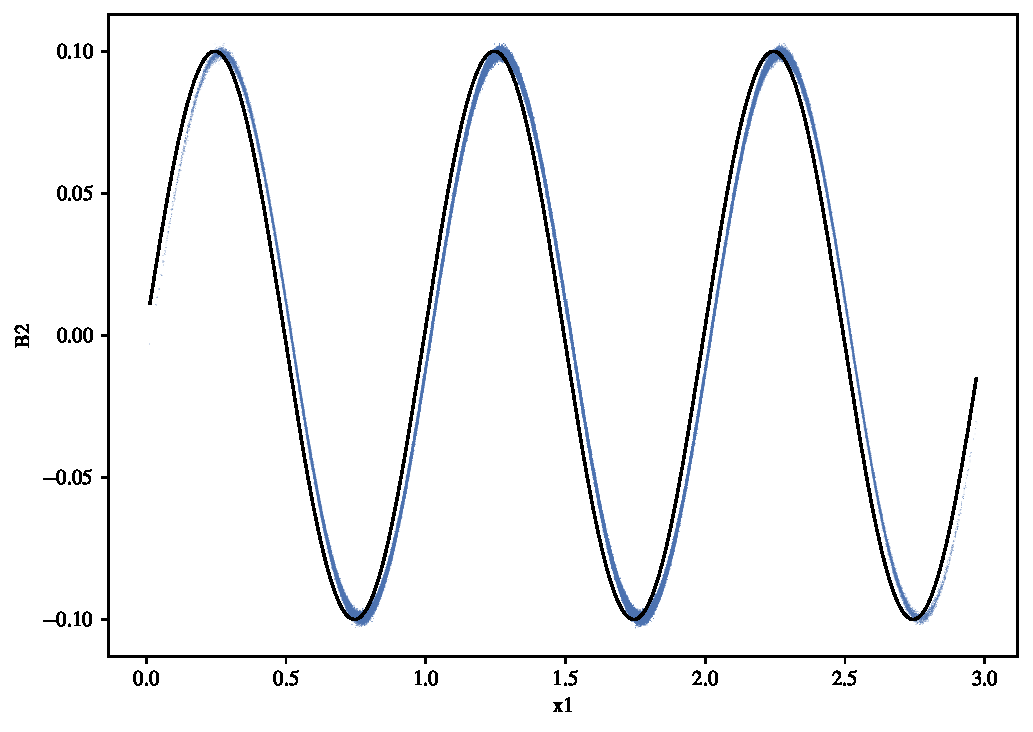
\includegraphics[width=0.45\linewidth]{img/Alfven/alfven_b2_step6_seaborn.pdf}
    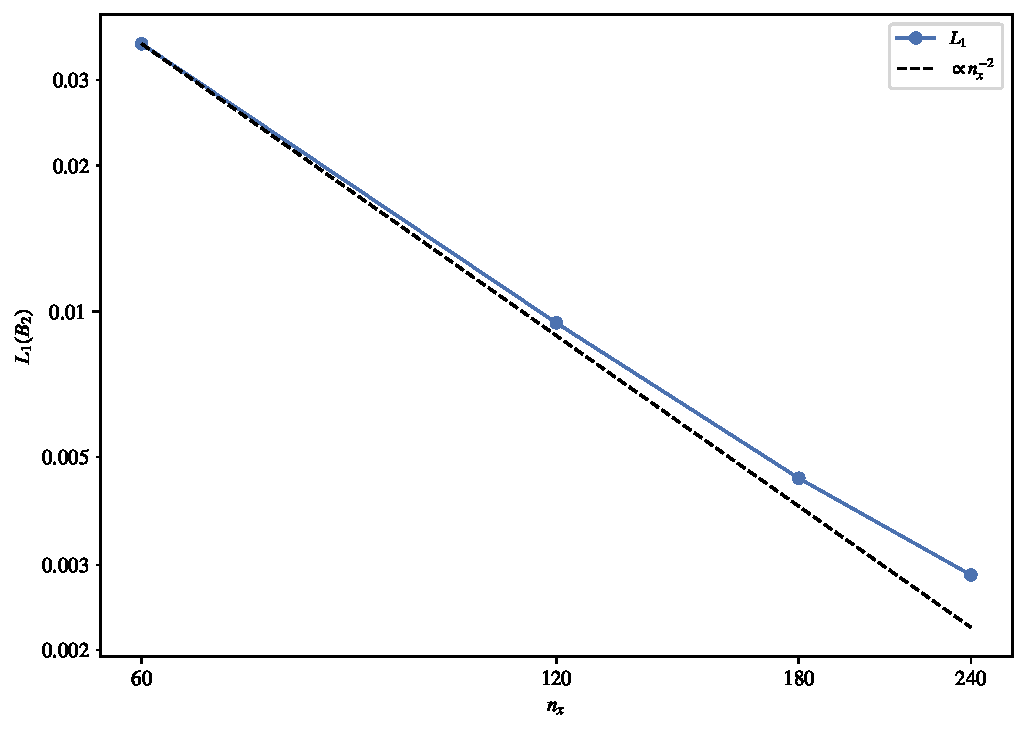
\includegraphics[width=0.45\linewidth]{img/Alfven/alfven_convergence.pdf}
    \caption{Results of the CP Alfvén Wave test. The first panel shows the particle magnetic field at $t=5$ projected onto the transverse axis $B2$ and scattered against position along the propagation direction $x_1$ (result for $120\times 60\times 60$ particles). The analytical solution (initial condition) is shown in black. The second panel shows the L1 error $L_1(B_2)$ as a function of resolution $n_x$, which converges with second-order.}
    \label{fig:alfven}
\end{figure}

\paragraph{Noisy Alfvén wave}
We present a slight modification of the Alfvén wave test not present in the reference literature, specifically to evaluate the performance of SLR. Additionally to the classic setup defined above, we add positionally-seeded white-noise perturbation to the magnetic field $B$ and velocity field $v$ in the initial conditions. With this we aim to observe how different dissipation schemes tackle incoherent noise (unresolved structure) versus the coherent wave (resolved structure). As described in §\ref{sec:slr}, the hope for SLR is to use full dissipation on the former while being able to linearly reconstruct and thus preserve the latter. 

To quantify this we perform a least-squares fit of the mode to both transverse components $B_2$ and $B_3$, and decompose the error into three errors: 
\begin{samepage}
\begin{itemize}
    \item Amplitude bleed: The ratio $A/A_0$ of the fitted mode amplitude $A$ to the initial $A_0=0.1$ to isolate resolved structure dissipation. 
    \item Phase error: The fitted phase minus the analytic phase to isolate dispersion. 
    \item $\delta B_n$: RMS of the mode subtracted transverse field to measure leftover noise perturbation.
\end{itemize}
\end{samepage}

Figure \ref{fig:alfven_noise} analyzes the results and compares different resistivity schemes. While both schemes perform well, SLR wins out in both conserving the resolved structure (amplitude) and in dissipating unresolved, uncorrelated noise. 

%better distinguish between these two types and, in this case where shocks are absent, to only dissipate the components of $B$ belonging to the former. 
% SW is also noisier, just mention quickly, already rejected concept anyways. 

\begin{figure}[h]
    \centering
    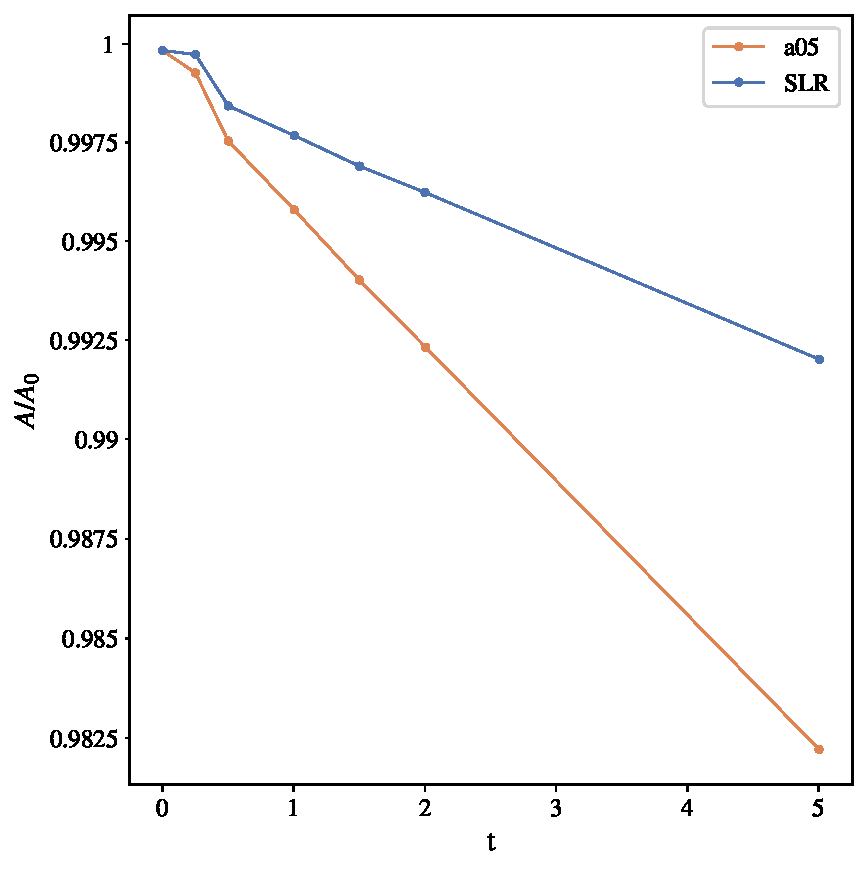
\includegraphics[width=0.33\linewidth]{img/Alfven/noise/alfven_analysis_amp.pdf}
    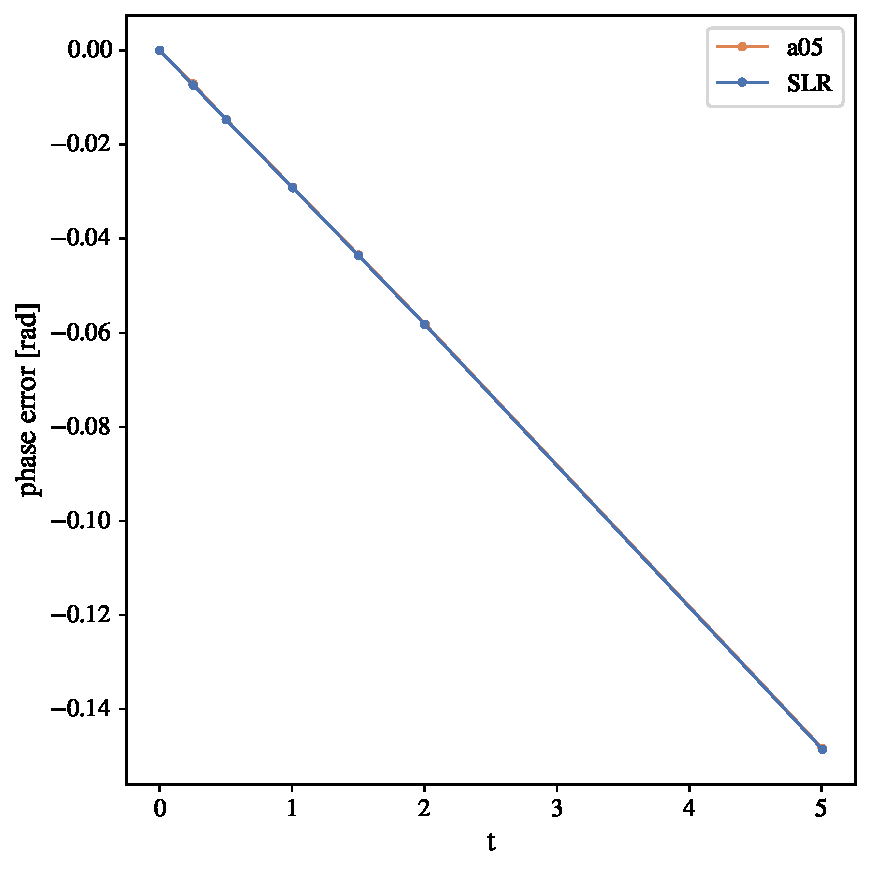
\includegraphics[width=0.33\linewidth]{img/Alfven/noise/alfven_analysis_phase.pdf}
    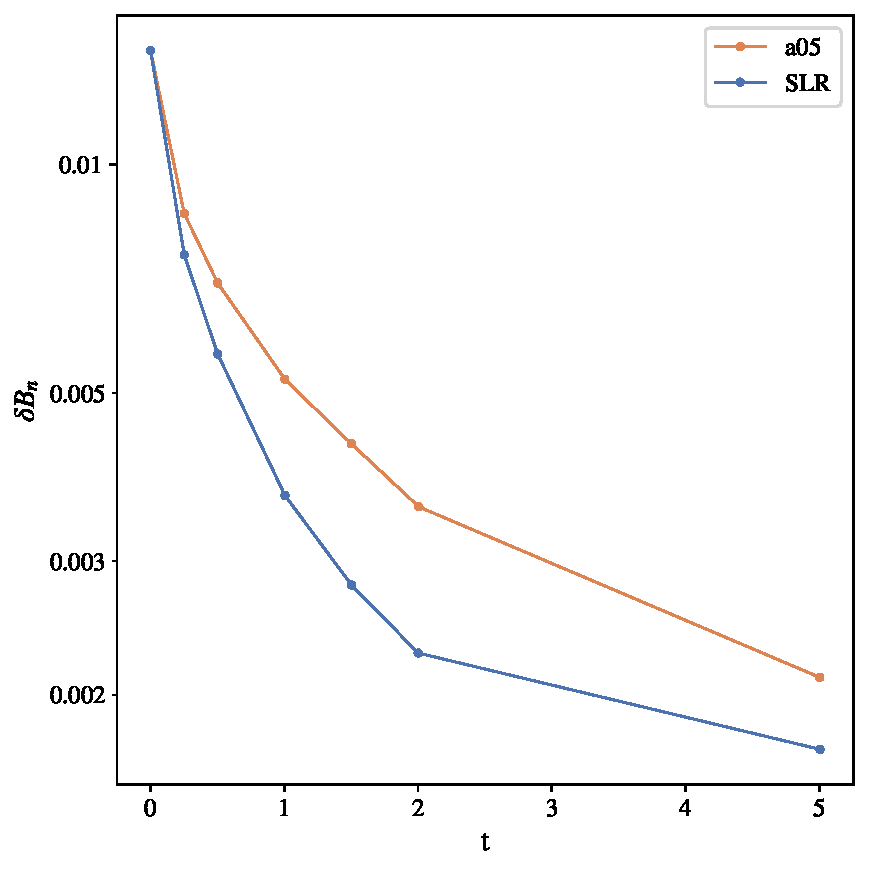
\includegraphics[width=0.33\linewidth]{img/Alfven/noise/alfven_analysis_noise.pdf} 
    \caption{Results of the noisy Alfven Wave (using noise amplitude \texttt{noiseAmp=0.01}) comparing a05 and SLR. First panel shows amplitude bleed $A/A_0$ over time, second panel shows phase error, and the last panel shows how fast the initial white noise is cleaned away. The phase error of both schemes is identical and the lines overlap completely. In the other panels we see that SLR slightly outperforms the baseline a05 in both directions: it shows \textit{less} dissipation when it comes to resolved structure (amplitude), but also better cleaning capabilities by dissipating \textit{faster} when it comes to unwanted noise.}
    \label{fig:alfven_noise}
\end{figure}

% \begin{figure}
%     \centering
%     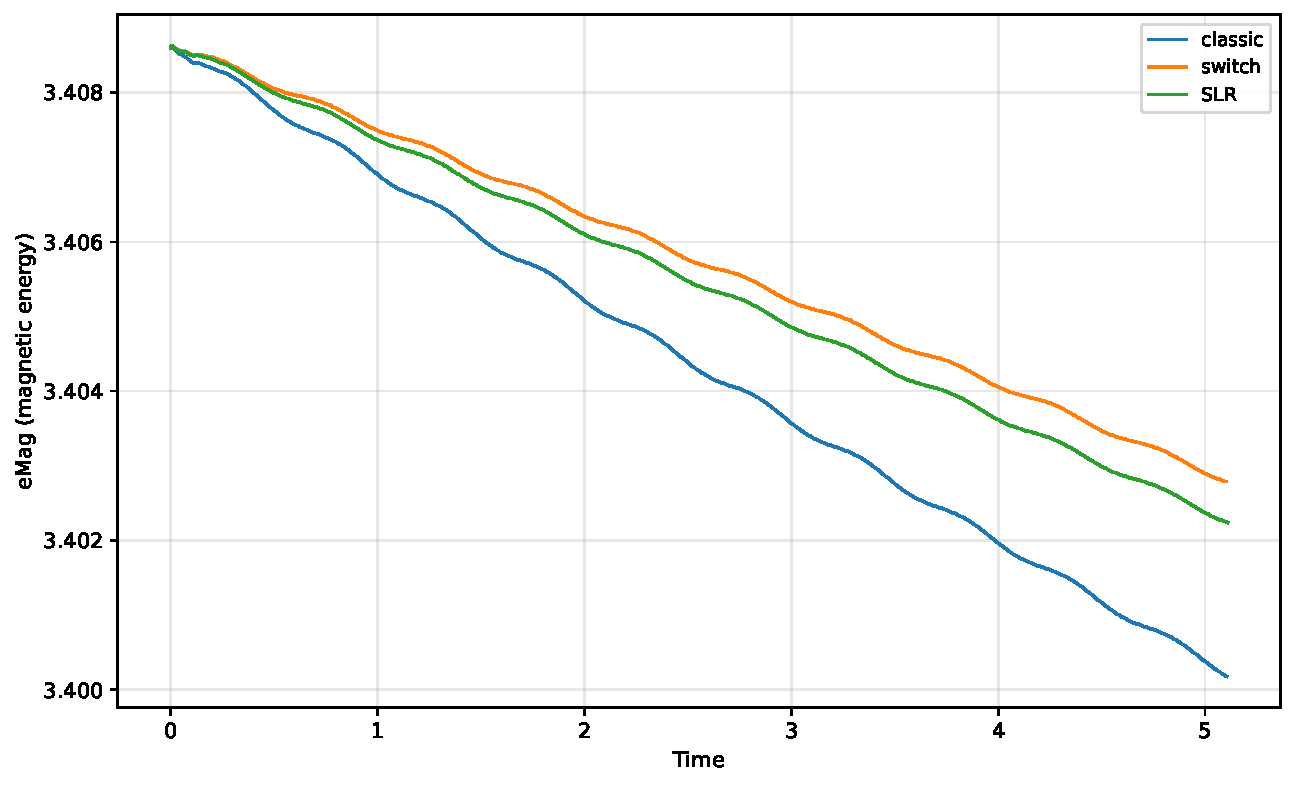
\includegraphics[width=0.8\linewidth]{img/Alfven/Alfven_wave_Emag_loss.pdf}
%     \caption{Loss of magnetic energy in Alfven wave test (remove, already got amplitude bleed)}
%     \label{fig:placeholder}
% \end{figure}


\subsection{Brio-Wu shocktube}
\label{sec:brio_wu}
The Brio-Wu shocktube is a simple extension of the Sod shocktube to MHD by applying a discontinuous magnetic field on top of the usual setup. It is designed to test how well SPMHD codes handle different shocks and discontinuities. In the context of resistivity schemes, it is our primary test of this verification suite to ensure that shocks are not under-dissipated (i.e. AR is not applied too weakly) which would result in overshoot and post-shock oscillations (see §\ref{sec:ar}). While there is no analytical solution to the Brio-Wu shocktube, we can use a reference solution calculated with a high-resolution grid code. 

We initialize a 3D thin periodic box of $[n_x,n_y,n_z] = [960, 60, 60]$ particles on the left side $[-2,0]$ and $[n_x,n_y,n_z] = [480, 30, 30]$ particles on the right side $[0,2]$ to get our desired density contrast of ratio $\rho_{left}/\rho_{right} = 8$. Field variables are initialized discontinuously as: 

$x\leq 0: \; (\rho_L, P_L, v_x, v_y, v_z, B_x, B_y, B_z) = (1, 1, 0, 0, 0, 0.75, 1, 0),\\
x > 0: \; (\rho_R, P_R, v_x, v_y, v_z, B_x, B_y, B_z) = (0.125, 0.1, 0, 0, 0, 0.75, -1, 0).$

The adiabatic index is $\gamma = 2$. We use constant AV (no switches, modulation or reconstruction) with $\alpha = 1.0$. This choice is made because we want to specifically evaluate the performance of the MHD implementation and not the hydro components. Constant AV improves the solution shape by reducing the amount of oscillations and overshoots compared to AVSLR or AVSW (switches). This way we can better isolate and compare the effects of AR schemes. 

Figure \ref{fig:brio_wu} shows the results after $t=0.2$. Particles within the active middle region $x\in [-1,1]$ are projected onto the $x$-axis. Additionally to the L1 error, each panel shows an \texttt{osc}-error, intended to measure post-shock ringing. It is defined as the maximum deviation from the reference solution $max(|q-q_{ref}|)$, but restricted to flat plateau areas of the solution where $|{dq_\mathrm{ref}}/{dx}|<0.2$. Additionally, these intervals are trimmed by $0.03$ off each end to exclude smeared shock-fronts. Both errors are calculated only over the window visible in Figure \ref{fig:brio_wu}.

SLR wins out slightly over the a05 baseline in most panels. Notably, showing slightly \textit{less} post-shock oscillation in $B_y$ while simultaneously also showing \textit{less} resistive heating $\dot u_\mathrm{diss}$. This seems counter-intuitive at shock fronts, but might point towards the fact that per-component dissipation is working as intended.

The results can be compared to Fig. 4 in \cite{WissingShen2020}, Fig. 28/29 in \cite{Price2018} and Fig. 2 in \cite{Hopkins2015}. Divergence errors show a higher floor than the comparisons, even before the shock-front, likely due to the velocity noise floor discussed at the beginning of §\ref{sec:numerical_tests}. 

Some hydro artifacts remain despite constant AV, such as the pressure spike around $x=0.1$ which also appears in pure hydrodynamic runs in SPH-EXA with magnetic forces disabled (reducing the test to the Sod shocktube). 

\begin{figure}
    \centering
    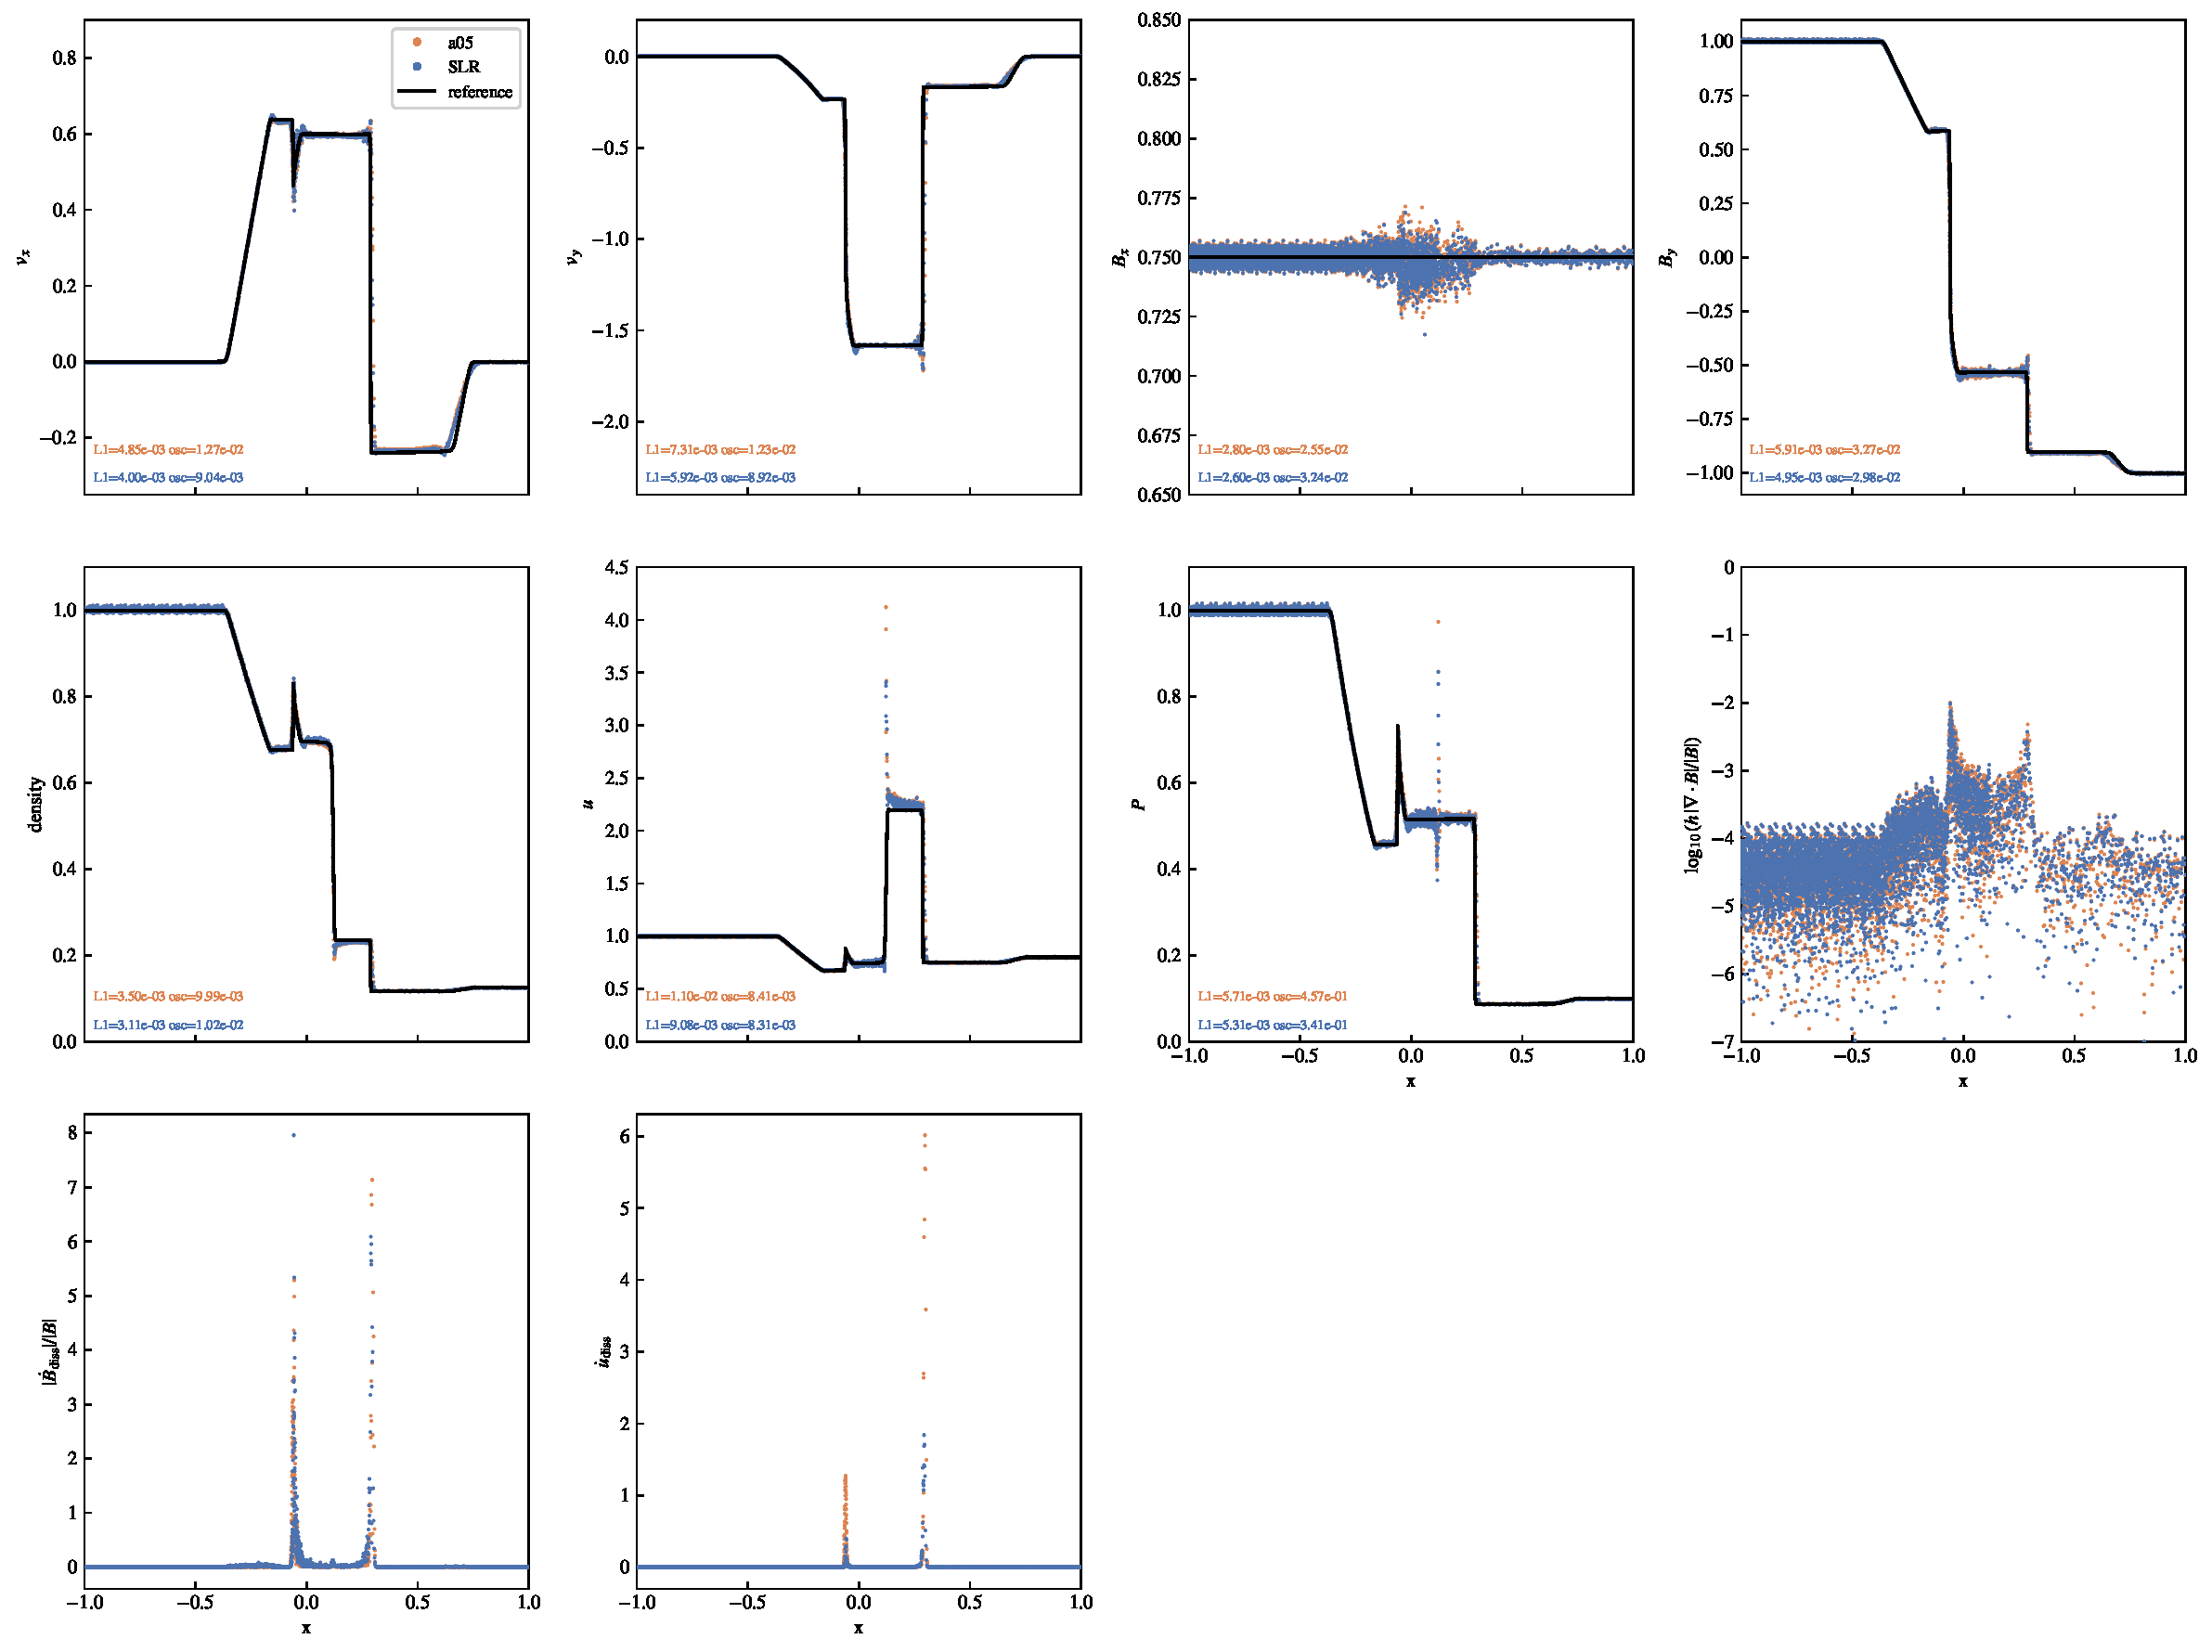
\includegraphics[width=\linewidth]{img/Brio-Wu/shocktube_compare_step2.pdf}
    \caption{Results of Brio-Wu shocktube: active region of the shock after $t=0.2$. Particles within $2\bar{h}$ ($\bar{h}$ the median smoothing length) of the box-axis are plotted against their $x$ position. Results of SLR are scattered as blue dots, those of a05 as orange dots. The reference solution is shown as a solid black line. We display nine field metrics in different panels, including their L1 error and \texttt{osc}-error (see §\ref{sec:brio_wu}) where applicable.}
    \label{fig:brio_wu}
\end{figure}

\subsection{Magnetized Sedov blast}
\label{sec:sedov}

In this magnetized blast wave we have a central, over-pressurized region which then expands preferentially along magnetic field lines instead of uniformly. This lets us i.a. test energy conservation under extreme pressure. 

A 3D square box $L=[1,1,1]$ is initialized with uniform density and resolution $N=250^3$. The inner region (radius $R=0.125$) is over-pressurized with $P_{in}=100$ while $P_{out}=1$). The initial magnetic field is set to $B = [10/ \sqrt{2}, 0, 10/\sqrt{2}]$, giving plasma beta $\beta_{in}=2$ and $\beta_{out}=0.02$. 

Figure \ref{fig:sedov} shows the results after $t=0.02$. Compared to Fig. 8 in \cite{WissingShen2020}, the bean-like shape of our blast wave appears a bit narrower with a slightly thicker shock front. The precise internal structure is hard to compare as their Fig 8. is a bit blurry (especially apparent when comparing the thermal pressure panel). We used same per-particle-h and kernel interpolation plotting method as described in the beginning of §\ref{sec:numerical_tests}. Overall however, we observe very similar solution structure. We also clearly see the expected double-shock in thermal pressure and the outer ring in the other three panels. 

Figure \ref{fig:sedov_metrics} shows that the conservation of total energy and the mean divergence error both improve with increasing resolution. Compared to the reported number of $\langle \varepsilon_{\text{divB}}\rangle=10^{-5}$ in \cite{WissingShen2020}, our divergence error is still one order of magnitude worse. 

\begin{figure}
    \centering
    % 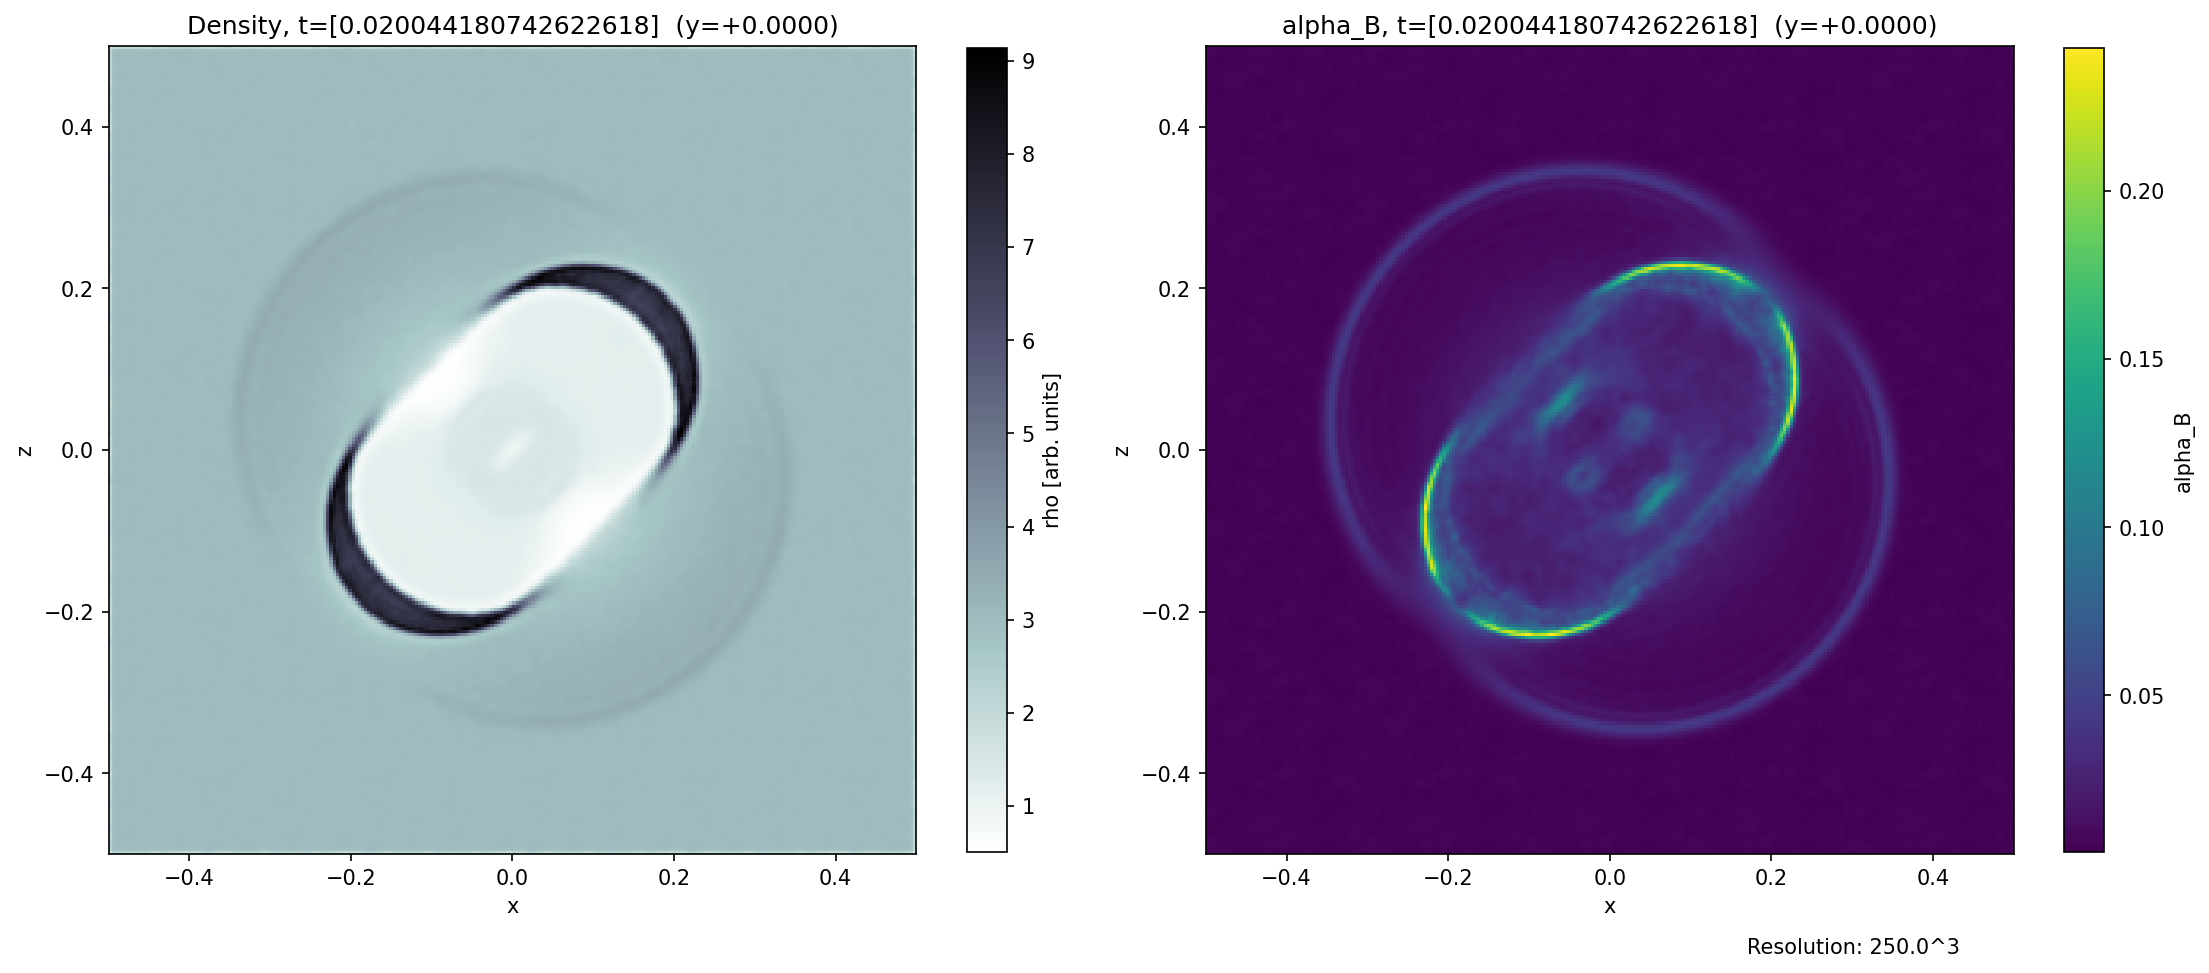
\includegraphics[width=0.8\linewidth]{img/sedov/slice_rho_step2_y+0.0000.png}
    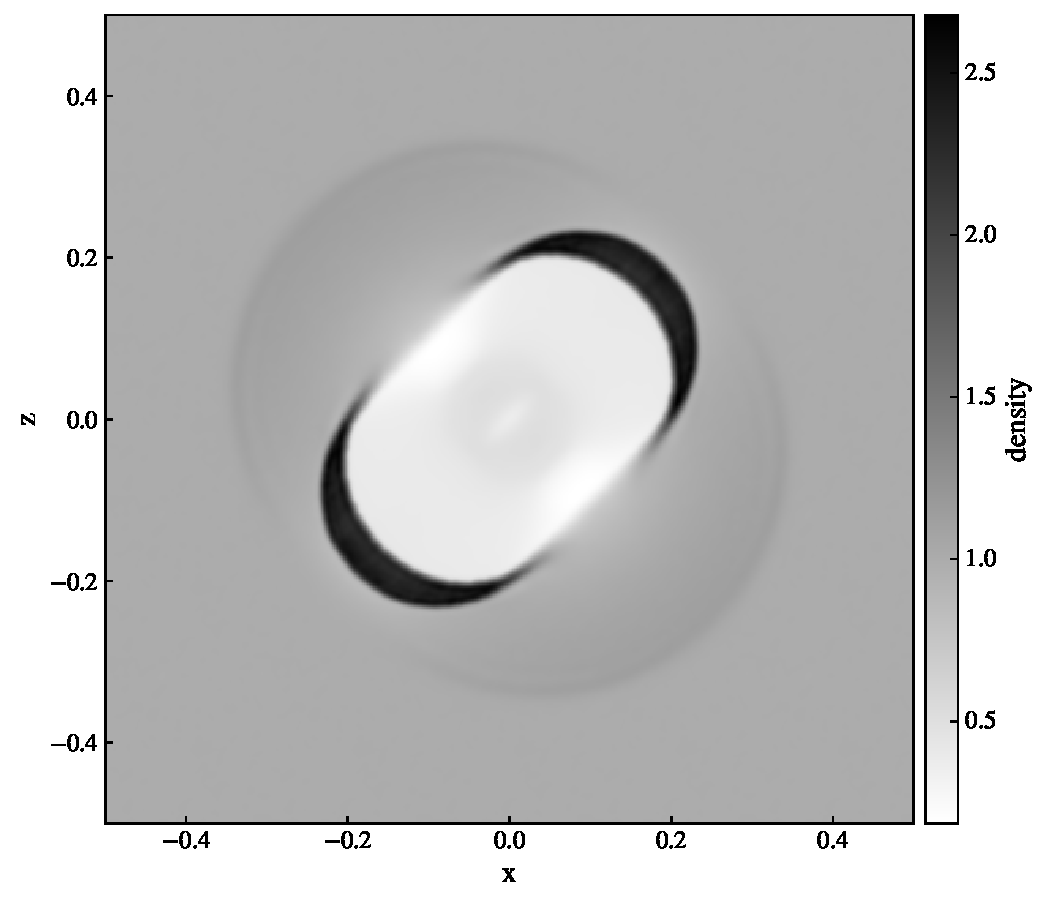
\includegraphics[width=0.49\linewidth]{img/sedov/slice_rho_step2_y+0.0000.pdf}
    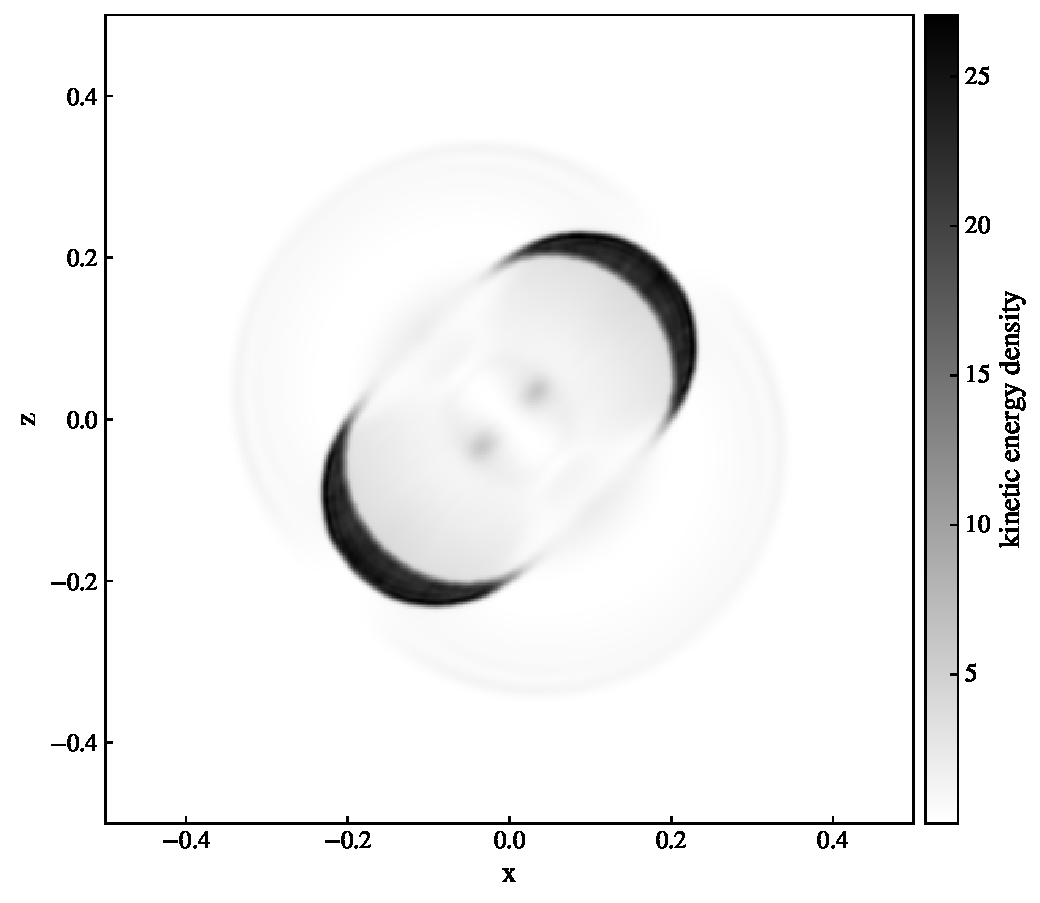
\includegraphics[width=0.49\linewidth]{img/sedov/slice_KE_step2_y+0.0000.pdf}
    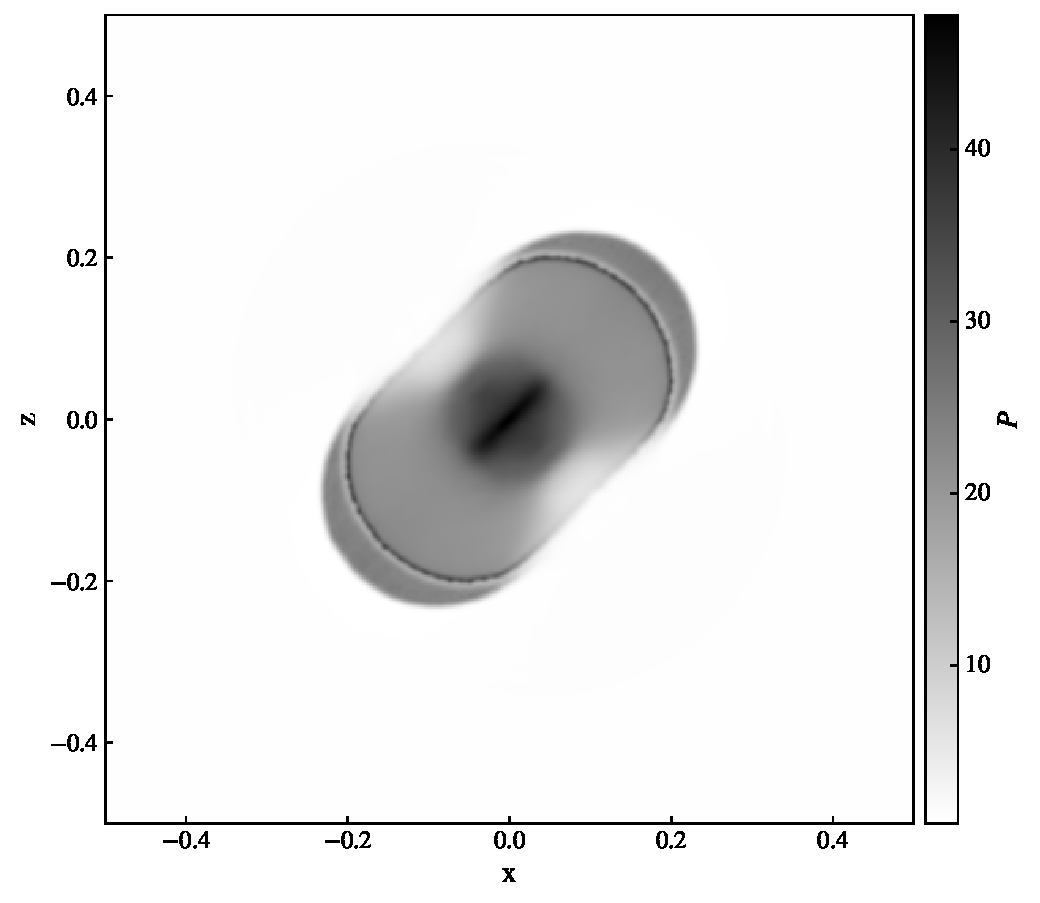
\includegraphics[width=0.49\linewidth]{img/sedov/slice_p_step2_y+0.0000.pdf}
    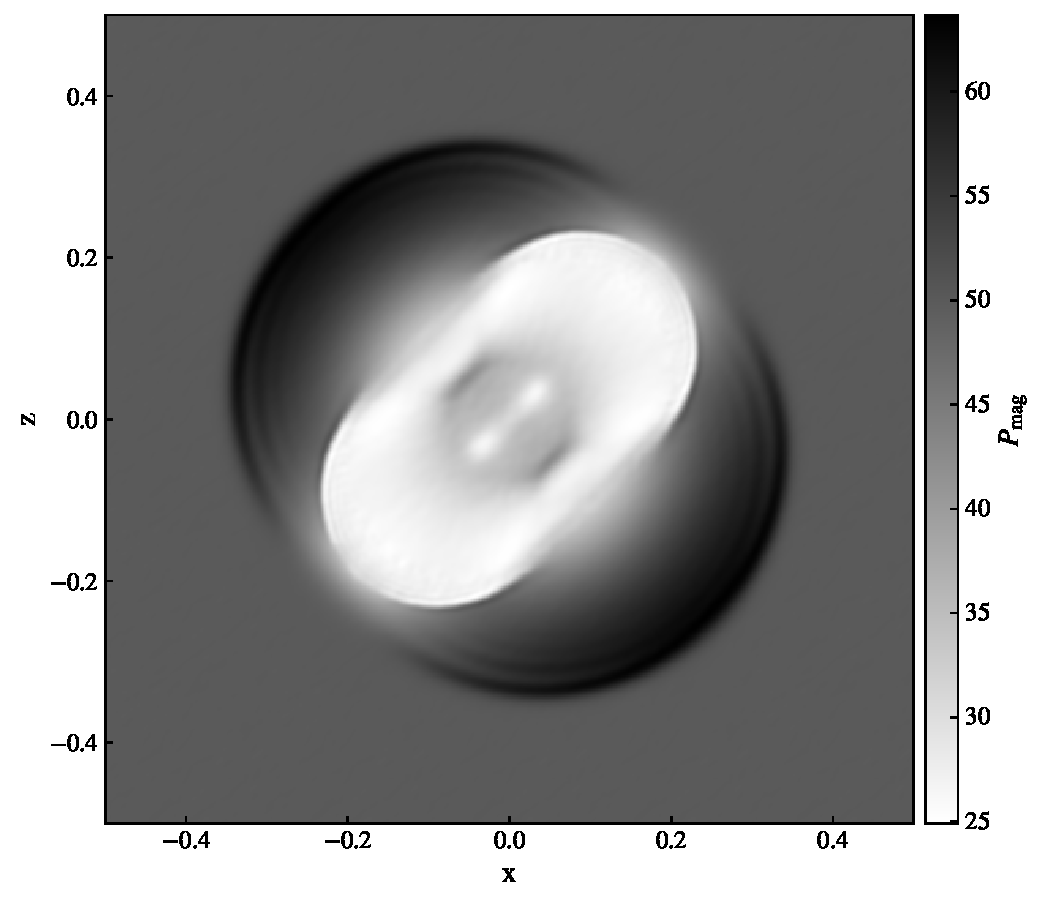
\includegraphics[width=0.49\linewidth]{img/sedov/slice_Pmag_step2_y+0.0000.pdf}
    \caption{Results of the magnetized Sedov blast with $N=250^3$ particles. Slices at $y=0$ and $t=0.02$ showing density (\textit{top left}), kinetic energy (\textit{top right}), thermal pressure $P$ (\textit{bottom left}), and magnetic pressure $P_{mag}$ (\textit{bottom right}).}
    \label{fig:sedov}
\end{figure}

\begin{figure}
    \centering
    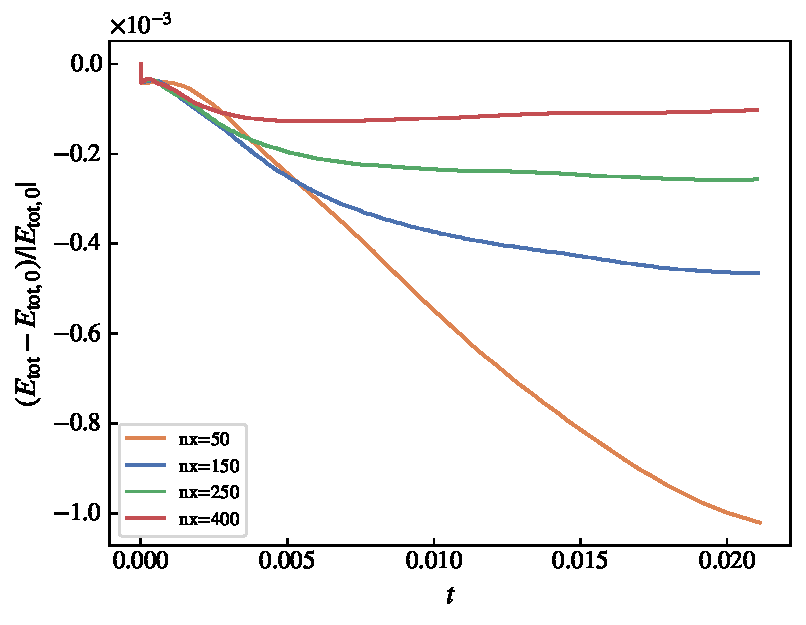
\includegraphics[width=0.4\linewidth]{img/sedov/compare_etot.pdf}
    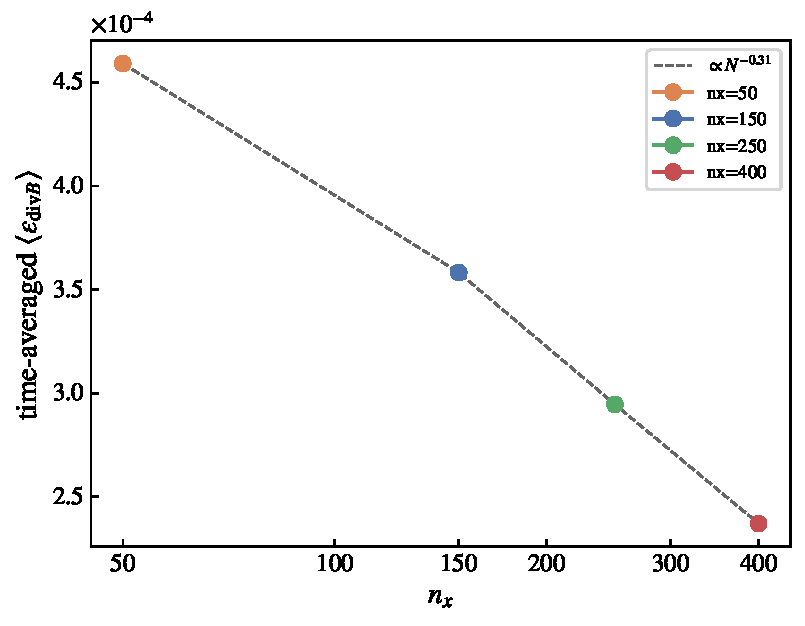
\includegraphics[width=0.4\linewidth]{img/sedov/compare_conv.pdf}
    \caption{Magnetized Sedov blast: Conservation of energy and evolution of divB error over time for different resolutions. The left panel shows the normalized total energy. An average run with $250^3$ particles stays within less than $0.3\%$ deviation. The right panel shows how the time-averaged mean divergence error decreases with increasing resolution $n$.}
    \label{fig:sedov_metrics}
\end{figure}

\todo[inline]{$N\rightarrow n$ or $\sqrt[3]{N}$}

\subsection{Current loop advection}
\label{sec:MHD_loop}

A weak magnetic loop is advected by a constant velocity field. The magnetic field is chosen small enough to be dynamically unimportant. In theory, the loop is thus expected to simply be moved along the velocity field and maintain shape throughout. This test is therefore great for determining numerical diffusion of the magnetic field. 

A thin periodic box is initialized with length $L=[2,1,\frac{30}{n_y}]$, velocity $v=[2,1,\frac{15}{n_x}]$, uniform pressure $P=1$, uniform density $\rho = 1$ and resolution $[n_x, n_y, n_z] = [120, 60, 30]$. The magnetic field inside the loop of radius $R_0=0.3$ is defined as ${B_0} = \frac{A_0}{r}(y, -x, 0)$ with $A_0=10^{-3}$. Outside the loop the magnetic field is zero. The loop is advected for $t=20$ periods. 

This test is especially susceptible to the velocity noise floor discussed in the beginning of §\ref{sec:numerical_tests}. The flow needed to conduct this test adequately needs to be uniform and almost perfectly smooth, which SPH-EXA with its glass-setup and kernel choice fails to deliver. Thus, the results are hard to compare against those in the reference papers using lattice initial conditions. 

Figure \ref{fig:loop_av_comp} compares four different runs, all using the same ARSLR scheme but combined with different AV schemes. It is clear that constant AV ($\alpha = 1$ with no switches, modulation or reconstruction) performs best at maintaining the loops shape, followed by AVSLR and lastly AVSW (AV switches). This is a direct consequence of how well each scheme smooths out the velocity field, specifically sub-resolution shear-noise. 

Constant AV is constantly tackling any kind of noise based on the approach velocity $\omega_{ab}$ of two particles (see eq. \eqref{eq:av_Pi}. AVSLR leaves sub-resolution shear noise largely undamped. Meanwhile AVSW reduces $\alpha$ close to $\alpha_{min}$ because switches only activate when there is compression. 

%AVSLR removes the resolved linear shear and therefore leaves sub-resolution shear noise largely undamped, which is why it ranks below constant AV here.

Remaining velocity noise leads to two effects via its small scale unphysical transverse flow: $E_{mag}$ injection by stretching the field (small scale dynamo via the induction equation \eqref{eq:induction}), and increased dissipation via the signal velocity $v_{\mathrm{sig},B} = |\mathbf{v}_{ab} \times \hat{\mathbf{r}}_{ab}|$ \eqref{eq:vsigB} used for resistivity \eqref{eq:ar_dB}. Two large noise driven terms which deteriorate the structure and violate conservation of magnetic energy in the direction of whichever term dominates. 

With this knowledge in mind, Figure \ref{fig:loop_ar_comp} uses constant AV to minimize the impact of velocity noise and then compares different AR schemes. Both a05 and SLR maintain the loop equally well, with the latter maybe showing marginally smoother interior and edges. A run using no magnetic dissipation ($\alpha_B=0$) is shown as reference. Figure \ref{fig:loop_metrics} then analyzes resistive heating and magnetic energy evolution of all three configurations with SLR winning out slightly over a05, showing $28\%$ less cumulative heating up to $t=20$.

\begin{figure}
    \centering
    % 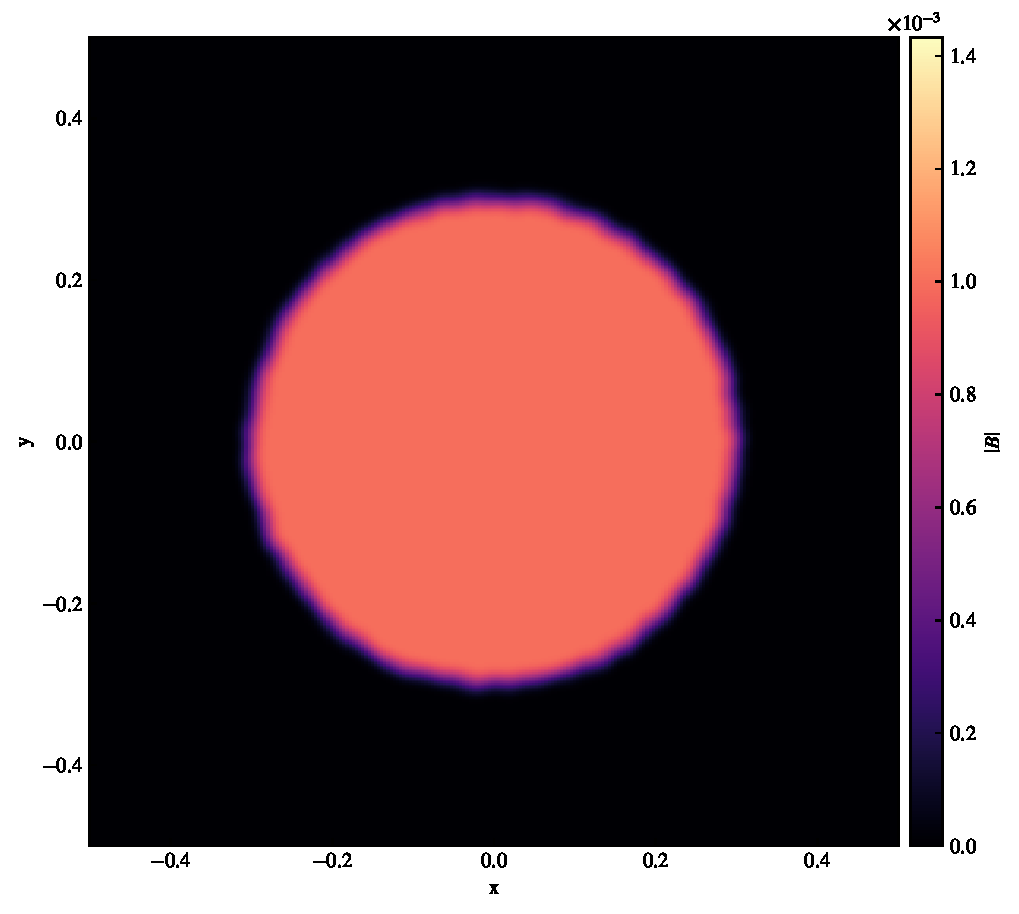
\includegraphics[width=0.49\linewidth]{img/MHD-Loop/INIT_slice_Bmag_step0_z+0.0000.pdf}
    % 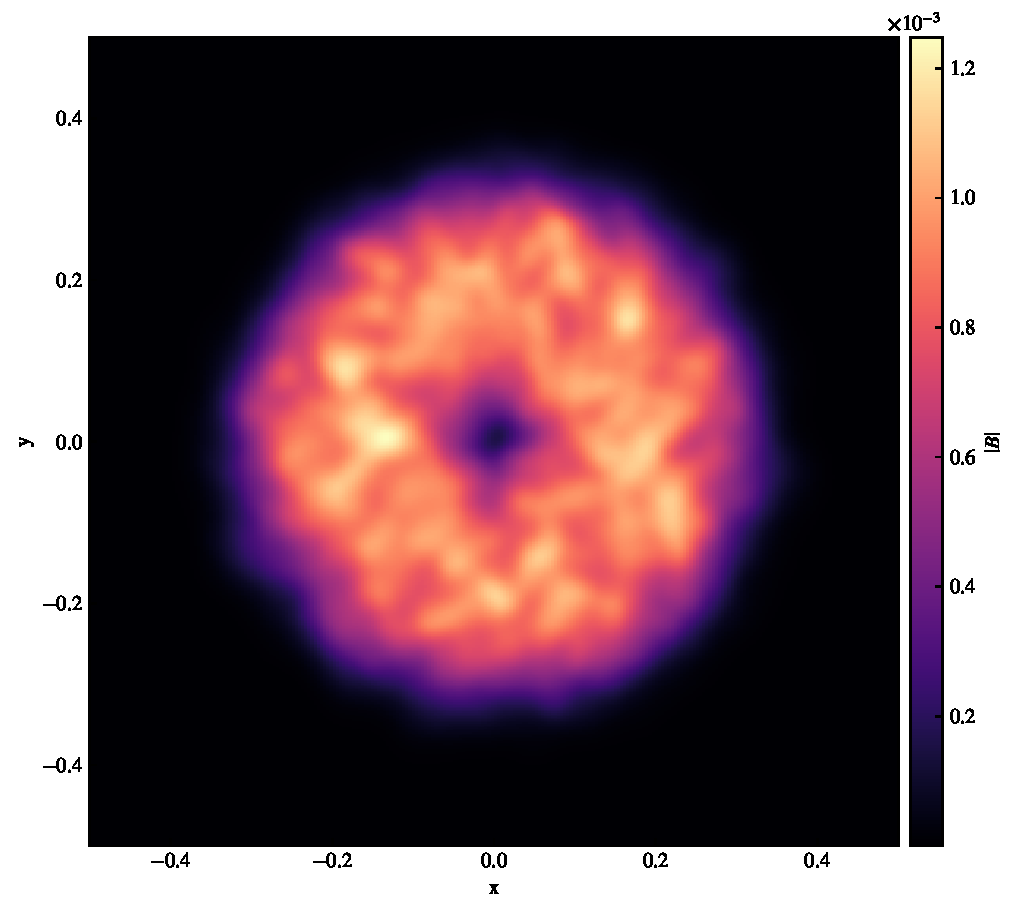
\includegraphics[width=0.49\linewidth]{img/MHD-Loop/AVSW_slice_Bmag_step3_z+0.0000.pdf}
    % 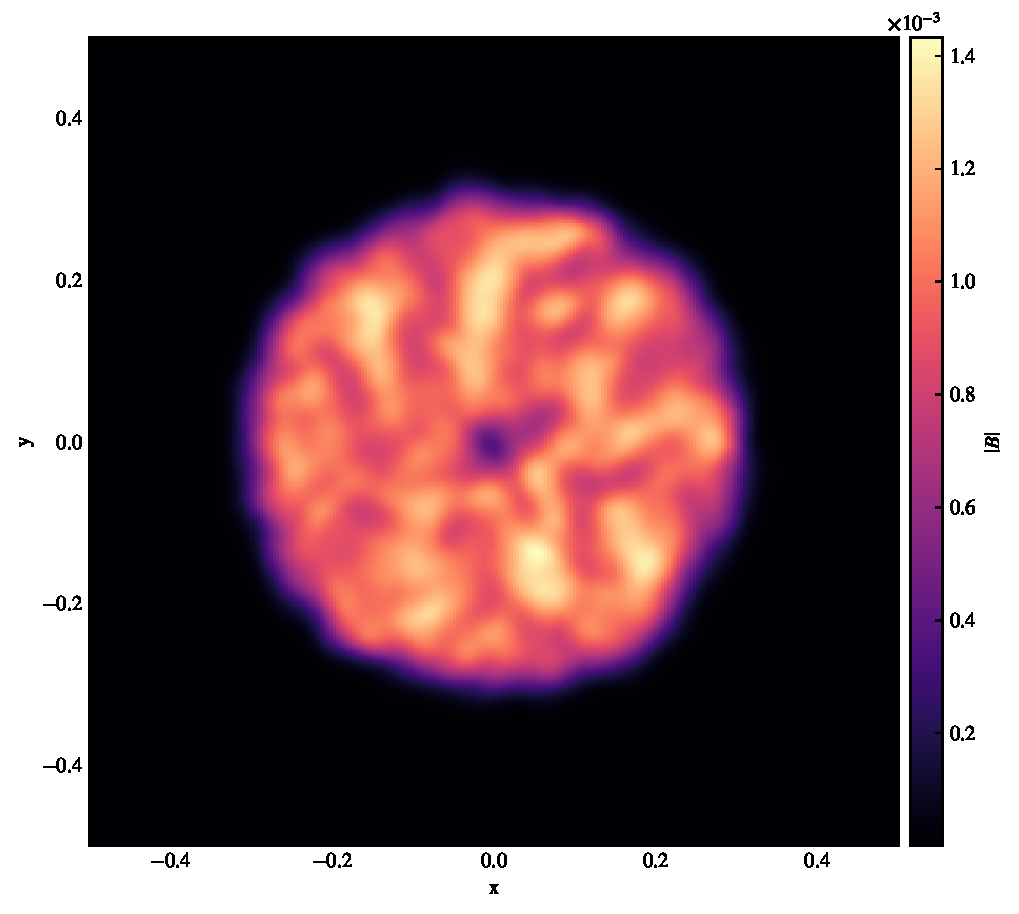
\includegraphics[width=0.49\linewidth]{img/MHD-Loop/AVSLR_slice_Bmag_step3_z+0.0000.pdf}
    % 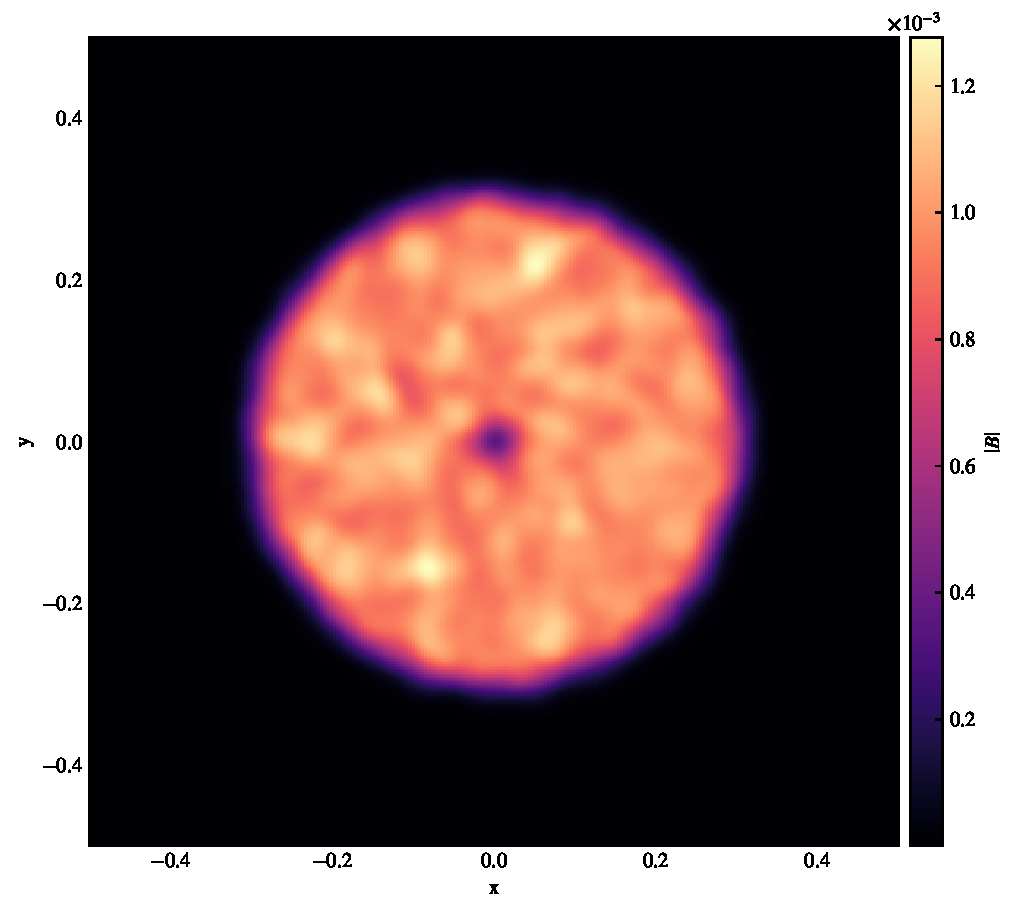
\includegraphics[width=0.49\linewidth]{img/MHD-Loop/AV_slice_Bmag_step3_z+0.0000.pdf}
    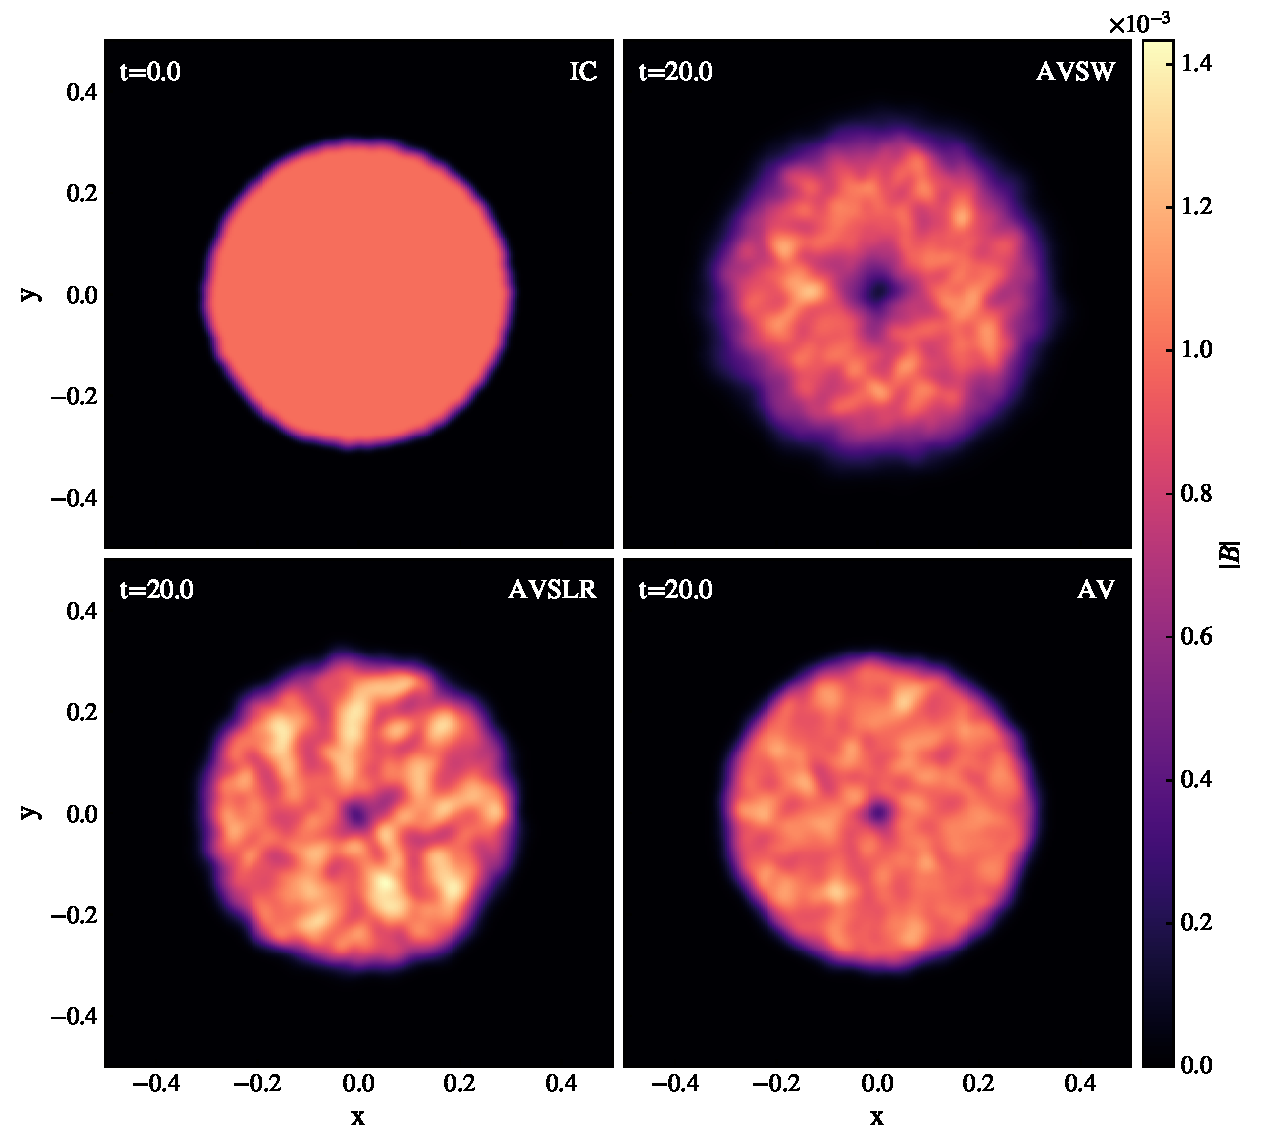
\includegraphics[width=0.8\linewidth]{img/MHD-Loop/slice_Bmag_step0_z+0.0000_panels.pdf}
    \caption{Results of the MHD advection loop showing slices of the magnetic field magnitude $|B|$: Initial condition (\textit{top left}) and results after t=20 periods using ARSLR together with three different AV schemes; AVSW (\textit{top right}), AVSLR (\textit{bottom left}) and constant AV $\alpha=1.0$ (\textit{bottom right}). Results using a05 produces almost identical results. The dominant factor in how well the loop structure is preserved in SPH-EXA, is how aggressively AV schemes smooth velocity noise $\delta v$ inherent to the flow.}
    \label{fig:loop_av_comp}
\end{figure}

\begin{figure}
    \centering
    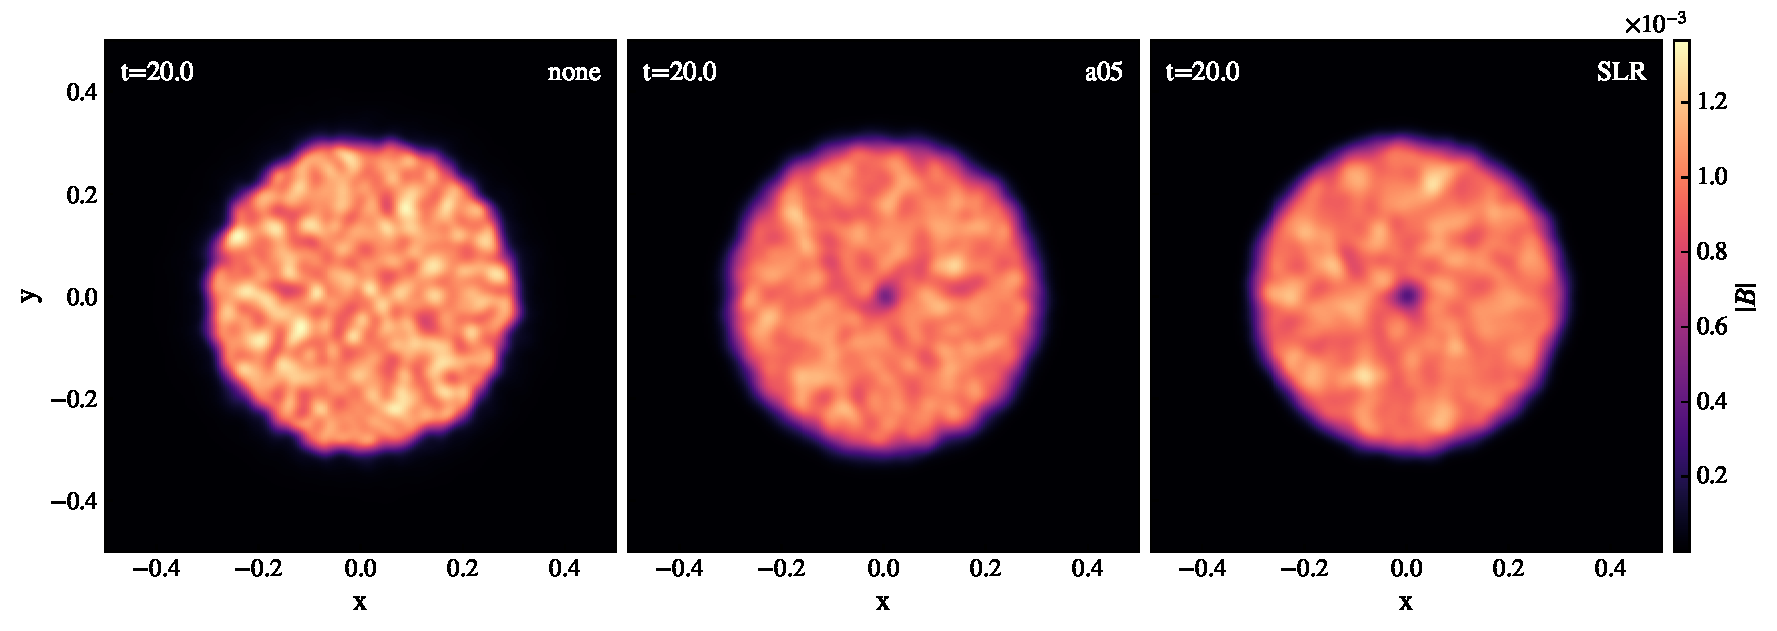
\includegraphics[width=\linewidth]{img/MHD-Loop/AR_scheme_slice_Bmag_step3_z+0.0000_panels.pdf}
    \caption{MHD advection loop using constant AV. Slices of magnetic field magnitude after $t=20$ for three different resistivity configurations (left to right): No AR ($\alpha_B=0$) vs a05 vs SLR.}
    \label{fig:loop_ar_comp}
\end{figure}

% \begin{verbatim}
% python sphexa/scripts/plot_slice.py out/9533596_SLR_avswitches/dump.h5 0 out/9533596_SLR_avswitches/dump.h5 3 out/7983967_Loop_SLR/dump.h5 3 out/9482508_Loop_SLR_noavslr/dump.h5 3 --clean --resolution 512 --label-time --labels IC AVSW AVSLR AV --cmap magma --xlim -0.5 0.5 --field Bmag
% \end{verbatim}

\begin{figure}
    \centering
    % 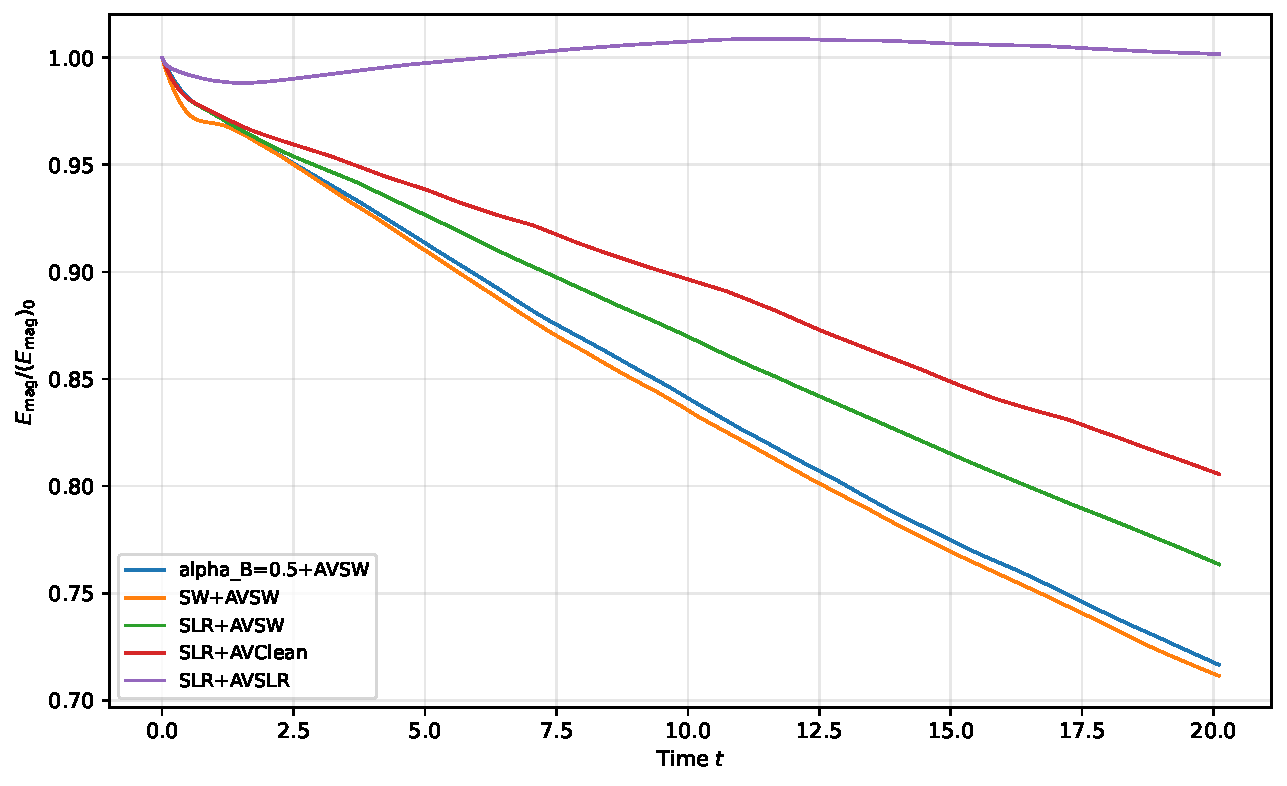
\includegraphics[width=0.8\linewidth]{img/eMagCompare/compare_eMag_4.pdf}
    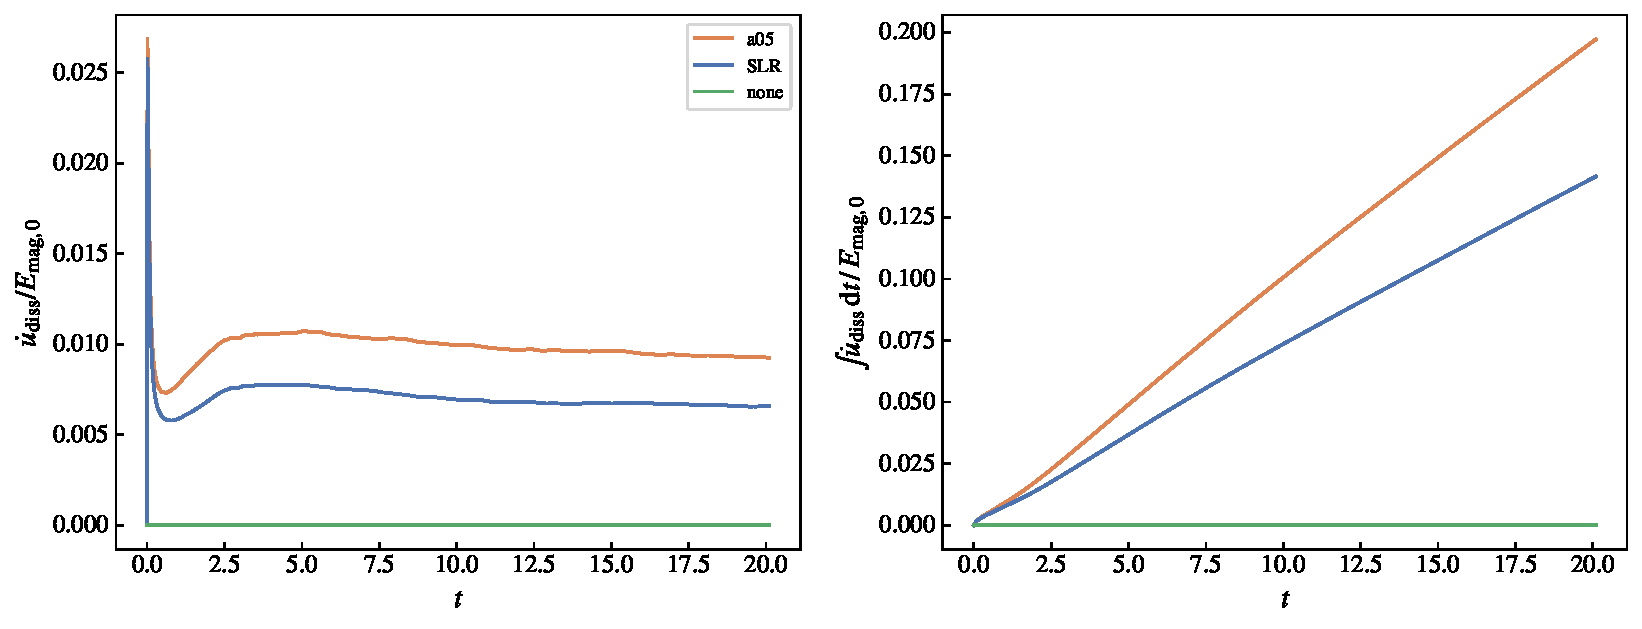
\includegraphics[width=\linewidth]{img/MHD-Loop/compare_heating.pdf}
    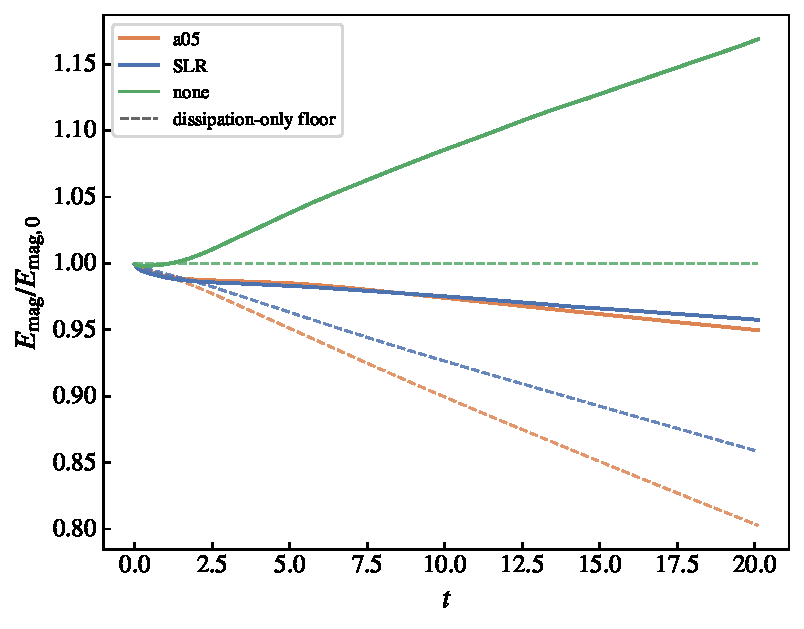
\includegraphics[width=0.5\linewidth]{img/MHD-Loop/compare_emag.pdf}
    \caption{Comparison of magnetic energy dissipation in the MHD advection loop using constant AV. The SLR scheme is shown in blue, a05 in orange, and a reference run using no AR ($\alpha_B=0$) in green. Top left panel shows normalized resistive heating rate $\dot u_{diss}$ over time. Top right panel shows the cumulative resistive heating. The bottom panel then compares the evolution of the normalized magnetic energy $E_{mag}/E_{mag,0}$. The dotted lines represent the evolution if the only change were through dissipation, while the solid lines represent the actual magnetic energy including dynamo-like stretching of field lines which increases the overall magnetic energy.}
    \label{fig:loop_metrics}
\end{figure}

\subsection{Orszag-Tang vortex}
The Orszag-Tang vortex \cite{Orszag1979} tests how well MHD codes handle transition to super-sonic turbulence  involves the development of super-sonic turbulence and multi-shock regimes where different shocks collide. It is therefore primarily a robustness and stability test. 

A thin periodic box of $L = [1, 1, \frac{30}{n_x}]$ is initialized with resolutions $[n,n,30]$ with $n\in\{120,240,510\}$. The initial velocity field and the doubly periodic magnetic field are set to:

$ [v_x, v_y, v_z] = v_0[-\sin(2\pi (y - y_{min})), \sin(2\pi (x - x_{min})), 0]$\\ 
$[B_x, B_y, B_z] = B_0[-\sin(2\pi (y - y_{min})), \sin(4\pi (x - x_{min})), 0],$

where $v_0=1$ and $B_0=1/\sqrt{4\pi}$. The initial plasma beta $\beta_0 = 10/3$ and Mach number $M_0=\frac{v_0}{c_s}=1$ and the usual adiabatic index $\gamma=5/3$ then give us our initial pressure $P_0=B_0^2 \beta_0 /2\approx0.133$ and density $\rho_0=\gamma P_0 M_0 \approx 0.221$.

Figure \ref{fig:ot_slices} shows the results after $t=0.5$ and $t=1.0$ for the three different resolutions. Comparing to Fig. 5 in \cite{WissingShen2020} and Fig. 32 in \cite{Price2018}, we manage to capture the overall structure well. With increasing resolution the shocks and the trapped high-density filament become visibly more defined. 

Figure \ref{fig:ot_linecuts} shows horizontal pressure slices to be compared with Fig. 33 in \cite{Price2018}. The profiles agree both qualitatively and quantitatively very well. One noticeable difference is a slight bump at $x\approx0.43$ in the second panel of our solution which is absent in theirs. With increasing resolution, the shock fronts become sharper. 

Figure \ref{fig:ot_divb} shows the behavior of the divergence error up until $t=3$. Both the mean and maximum error stay bounded, with the mean staying below $10^{-2}$, which was established as the preferable upper limit \cite{WissingShen2020}. It is important that we see a clear plateau emerging around $t=1.3$, meaning the error is source-limited rather than cleaning-limited. In the last panel of Figure \ref{fig:ot_divb} we see how the divergence error successfully declines with increasing resolution. 

% Robustness in multi-shock regime. Stability and divB cleaning (longer sim time?) when shocks collide. Density/pressure structure linecut vs reference. total energy drift. 

\begin{figure}
    \centering
    % 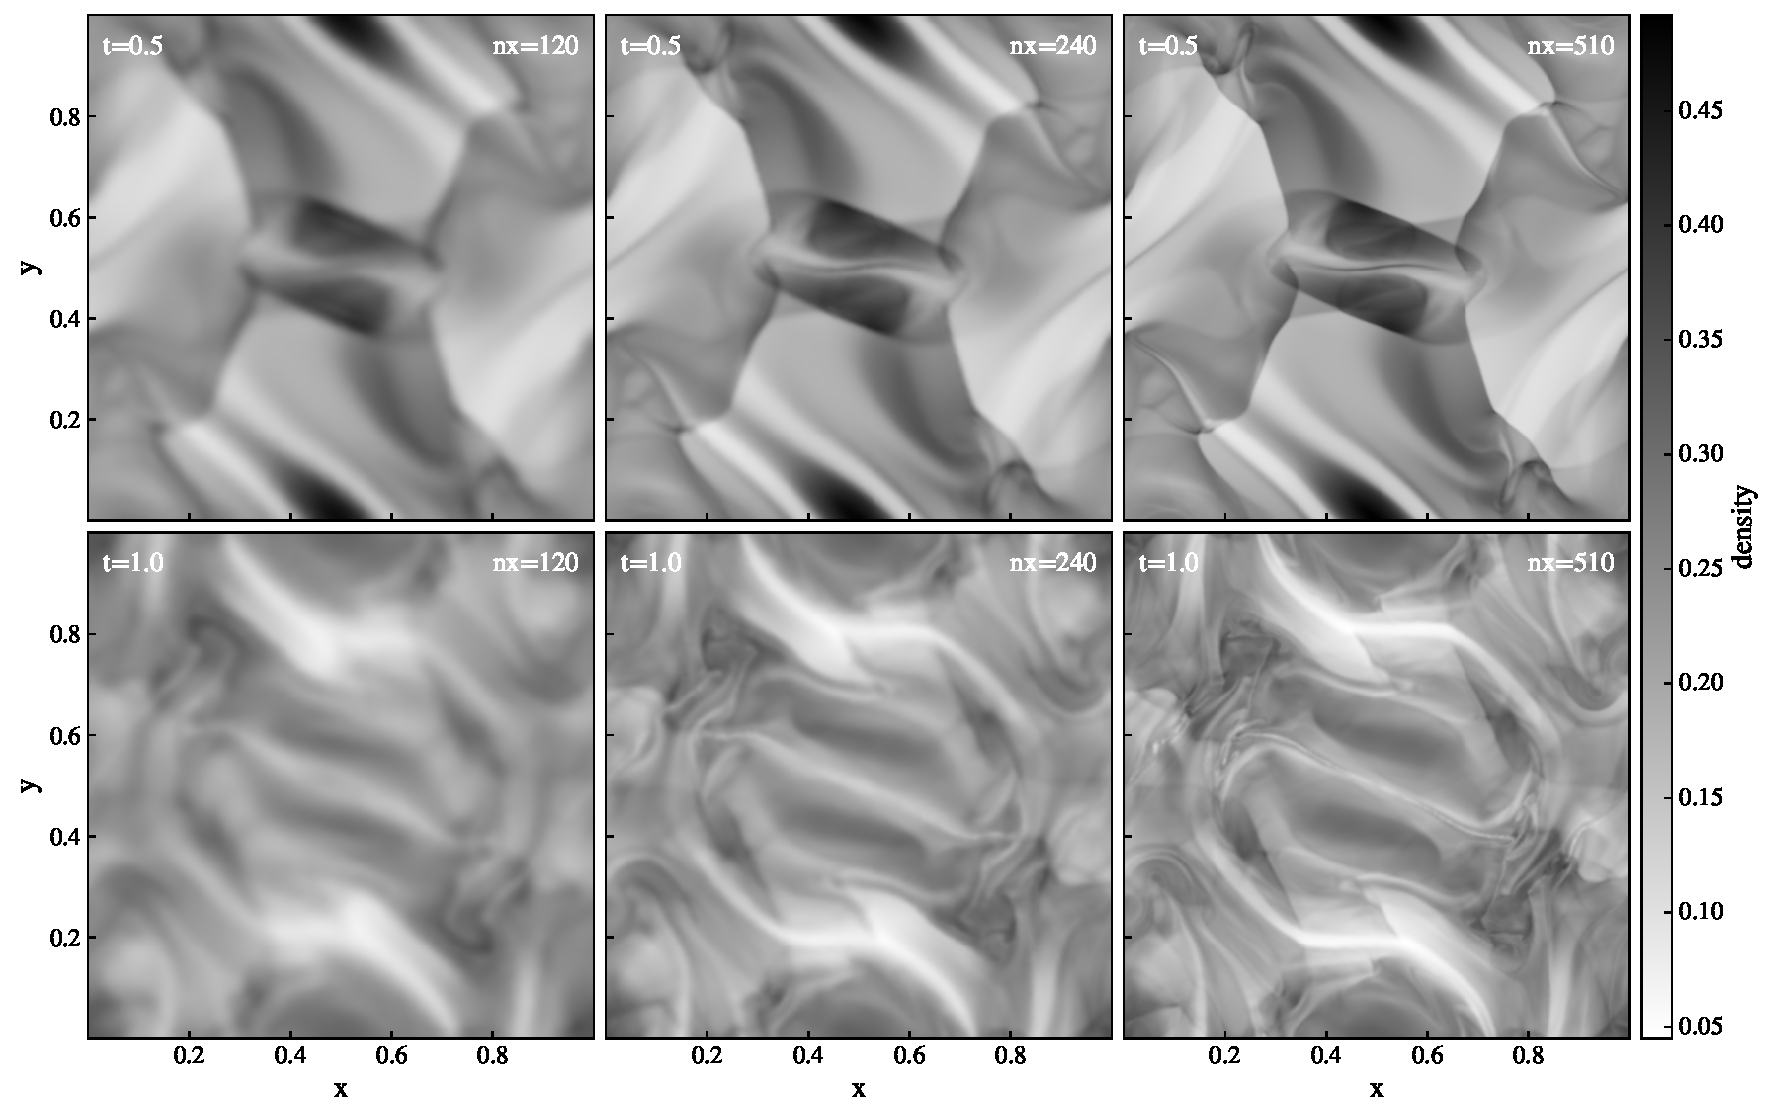
\includegraphics[width=\linewidth]{img/OT/gray_r_slice_rho_step1_z+0.0000_panels.pdf}
    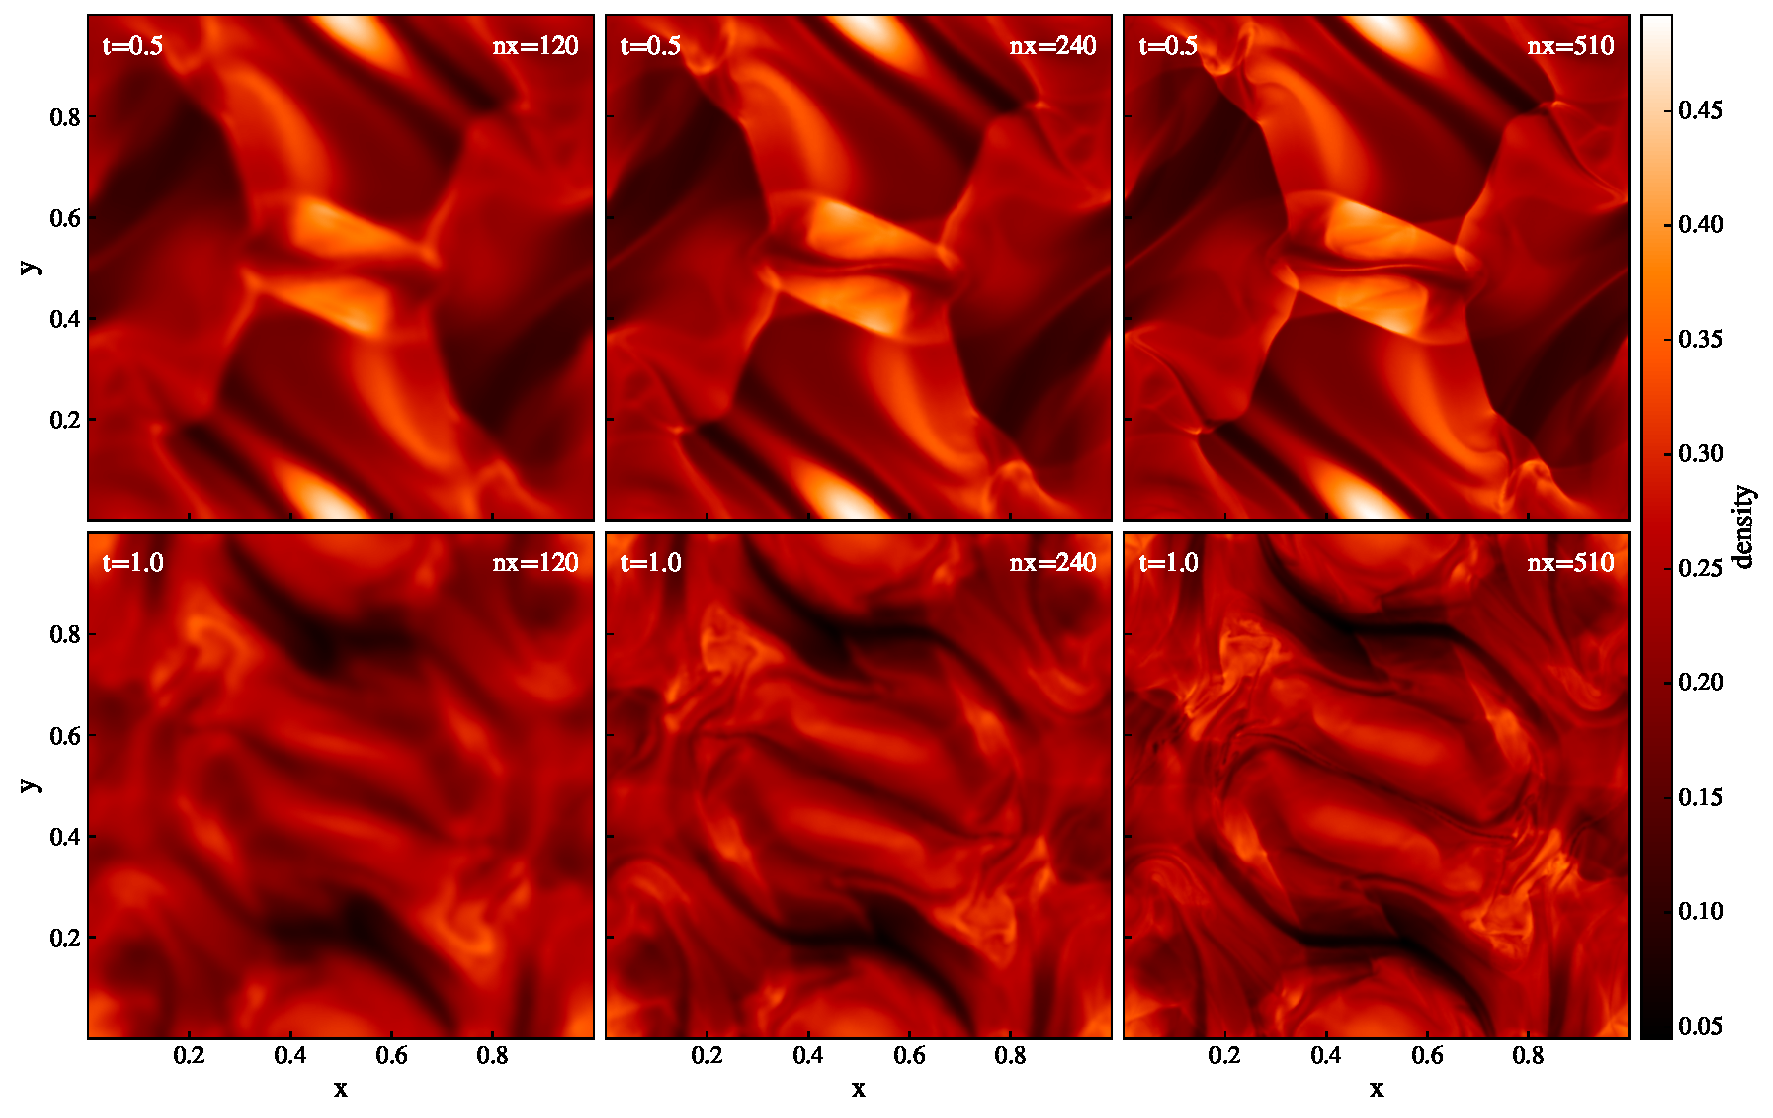
\includegraphics[width=\linewidth]{img/OT/slice_rho_step1_z+0.0000_panels.pdf}
    % 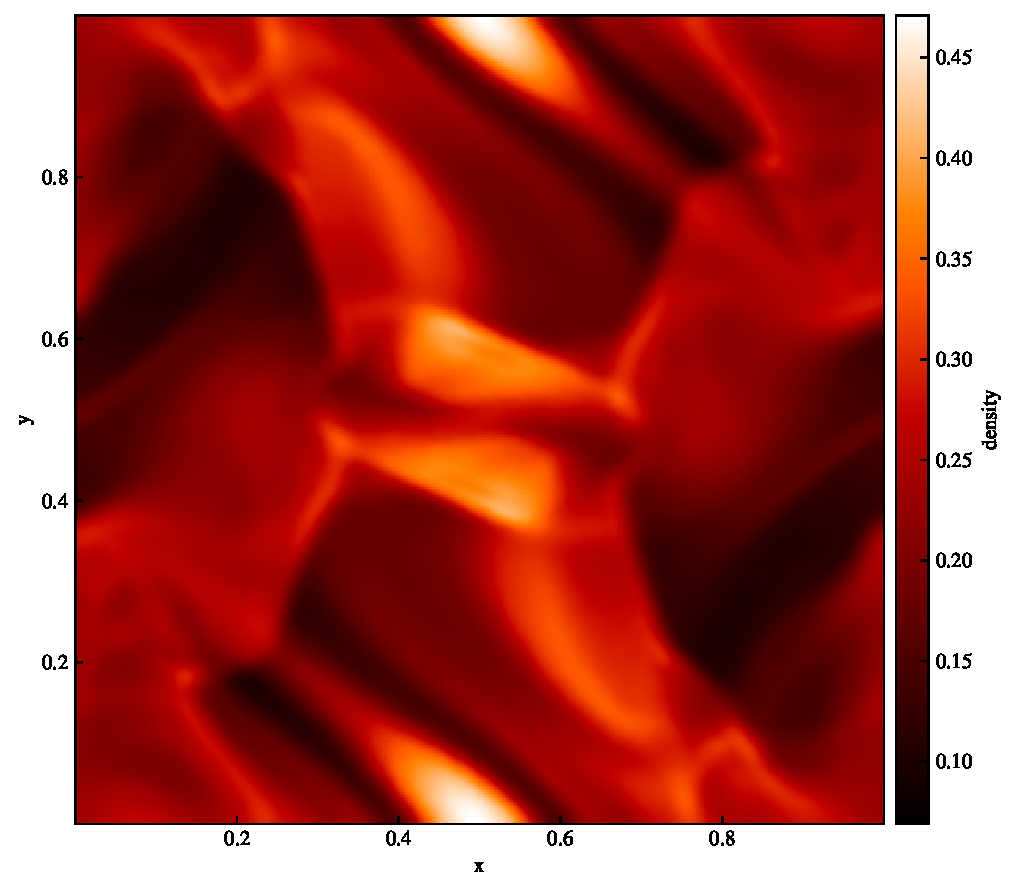
\includegraphics[width=0.49\linewidth]{img/OT/slice_rho_step1_z+0.0000_120.pdf}
    % 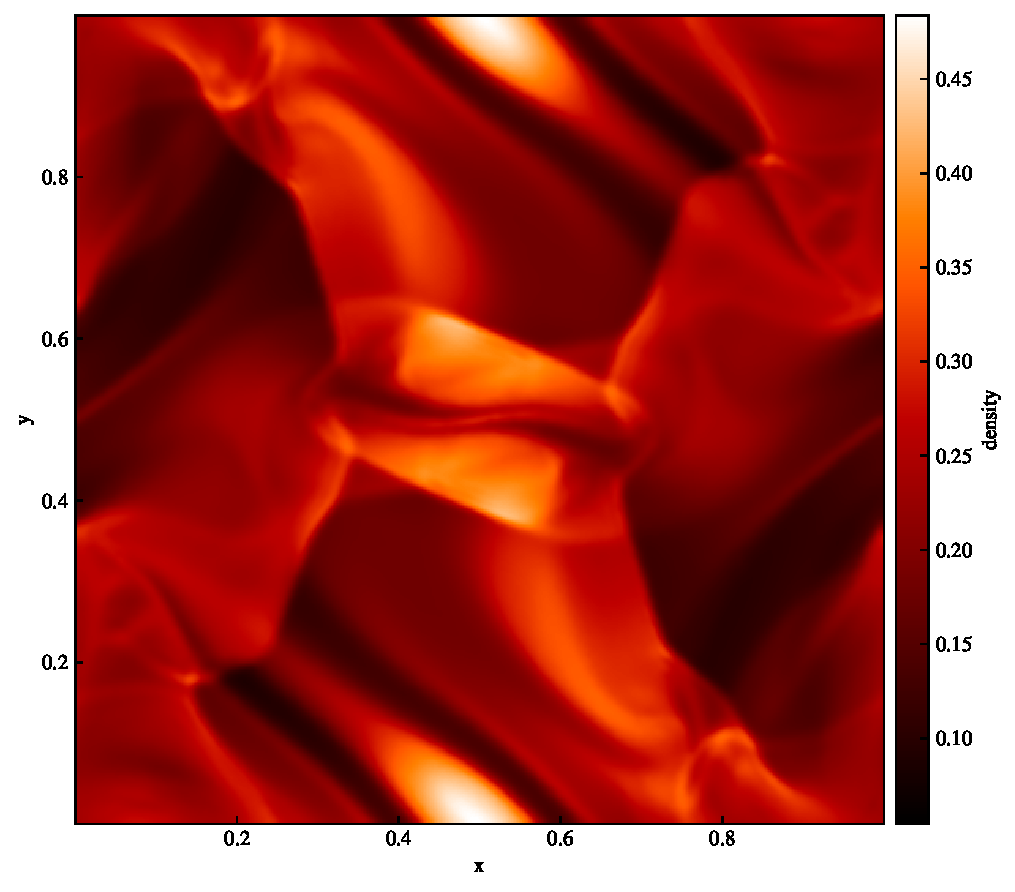
\includegraphics[width=0.49\linewidth]{img/OT/slice_rho_step1_z+0.0000.pdf}
    % 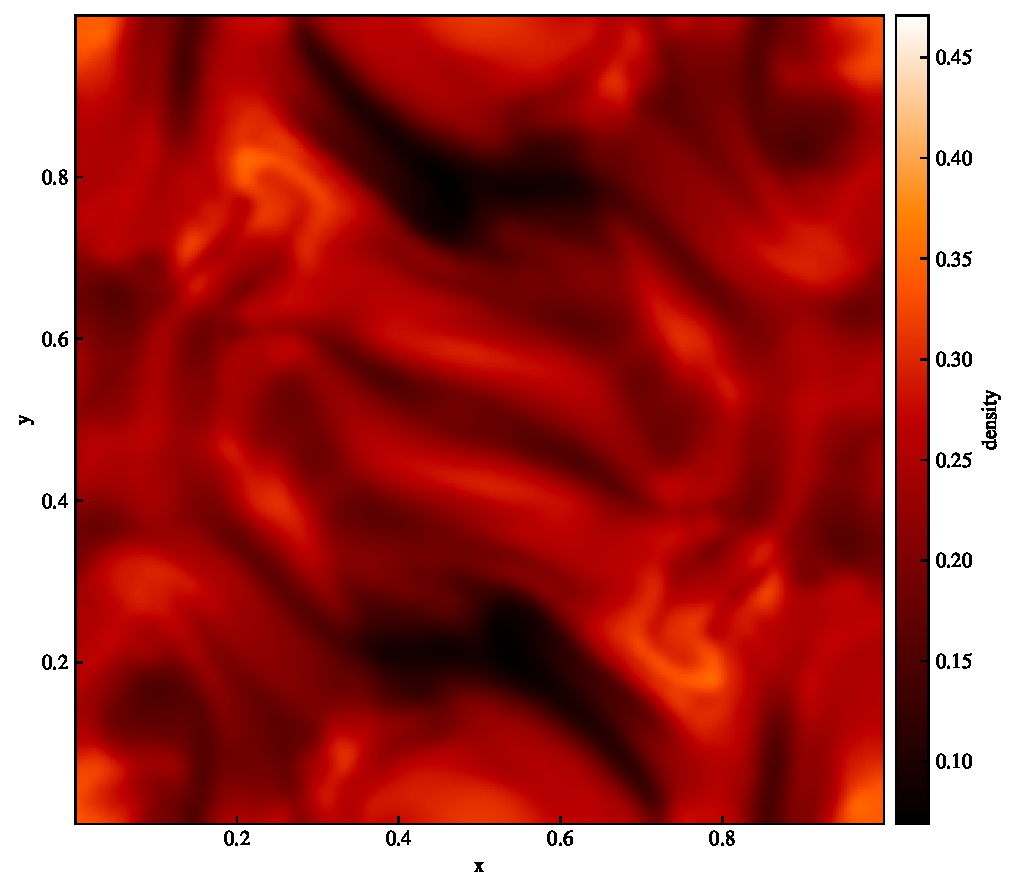
\includegraphics[width=0.49\linewidth]{img/OT/slice_rho_step2_z+0.0000_120.pdf}
    % 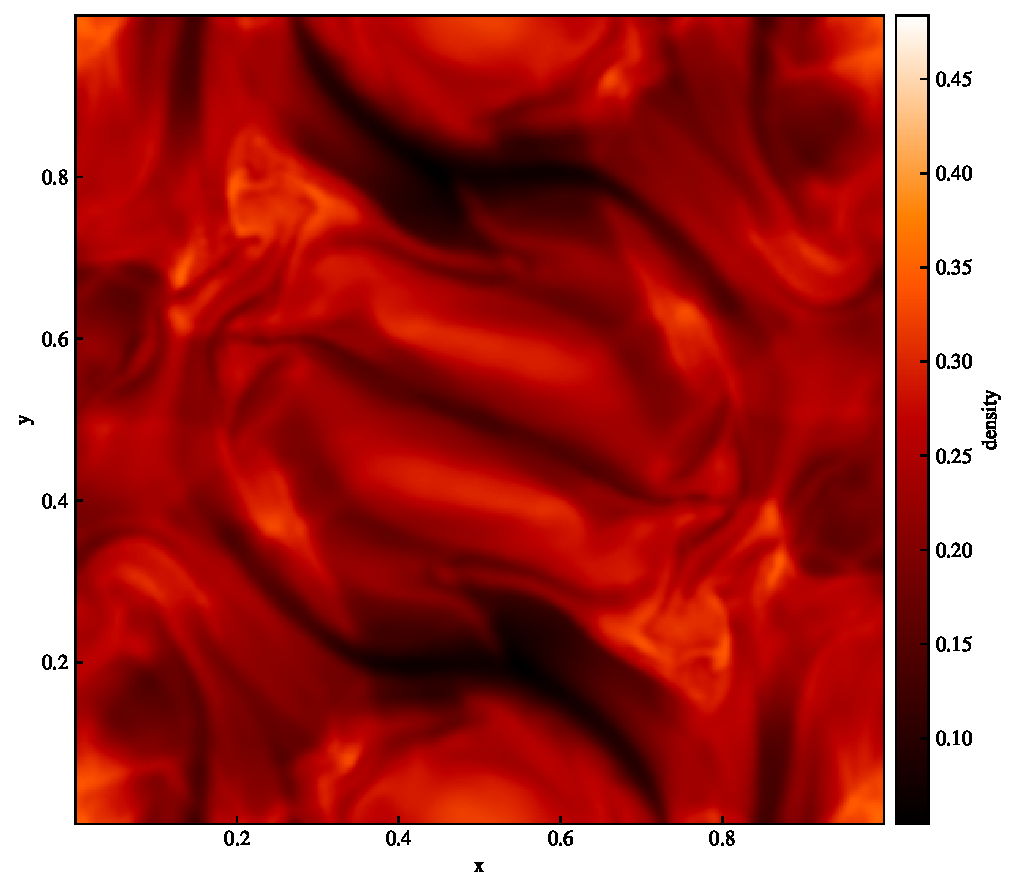
\includegraphics[width=0.49\linewidth]{img/OT/slice_rho_step2_z+0.0000.pdf}
    \caption{Results of the Orszag-Tang vortex. Density slices at $t=0.5$ (\textit{top}) and $t=1.0$ (\textit{bottom}). For three increasing resolutions $n_x\in\{120,240,510\}$ left to right.}
    \label{fig:ot_slices}
\end{figure}

\begin{figure}
    \centering
    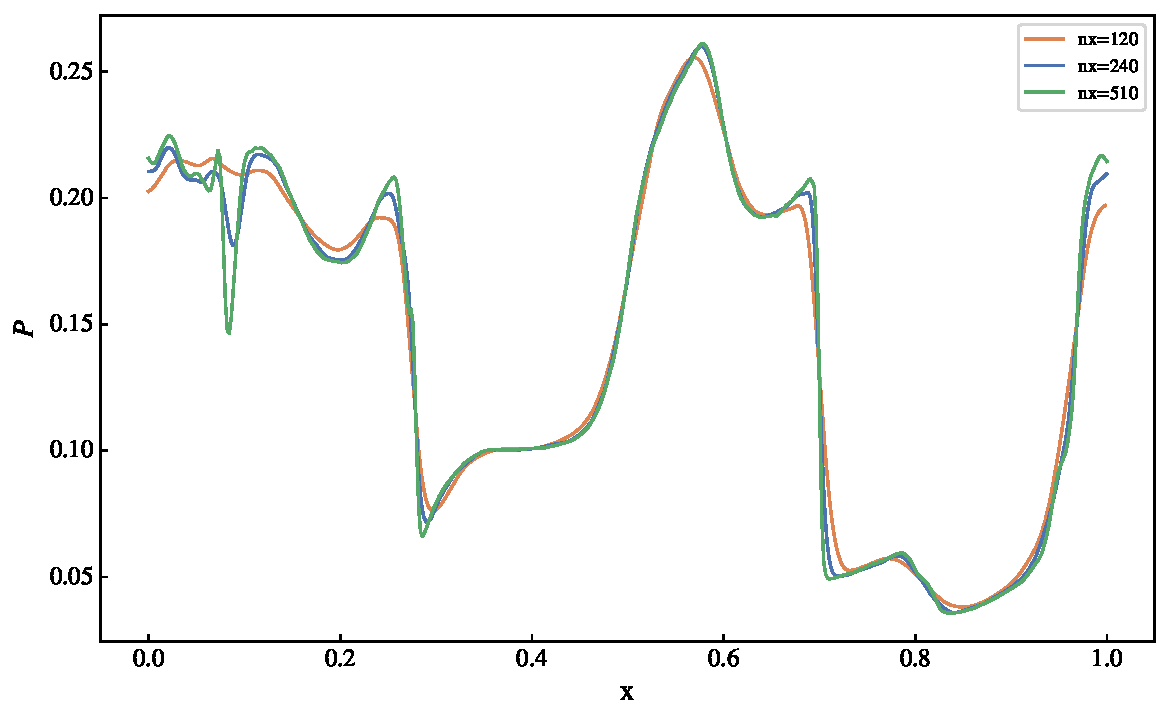
\includegraphics[width=0.4\linewidth]{img/OT/linecut_p_step1_x_y+0.3125_z+0.0000.pdf}
    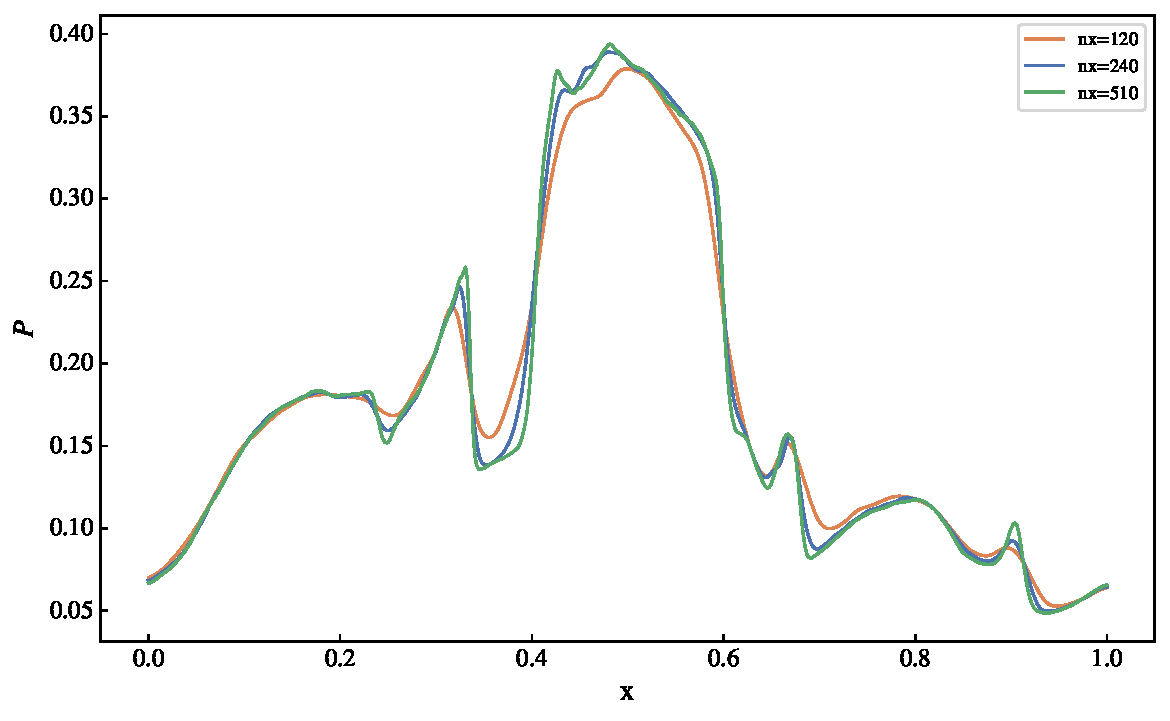
\includegraphics[width=0.4\linewidth]{img/OT/linecut_p_step1_x_y+0.4277_z+0.0000.pdf}
    \caption{Orszag-Tang vortex: Pressure slices at $t=0.5$ along $y=0.3125$ (\textit{left}) and $y=0.4277$ (\textit{right}) plane for different resolutions $n_x\in\{120,240,510\}$.}
    \label{fig:ot_linecuts}
\end{figure}

\begin{figure}
    \centering
    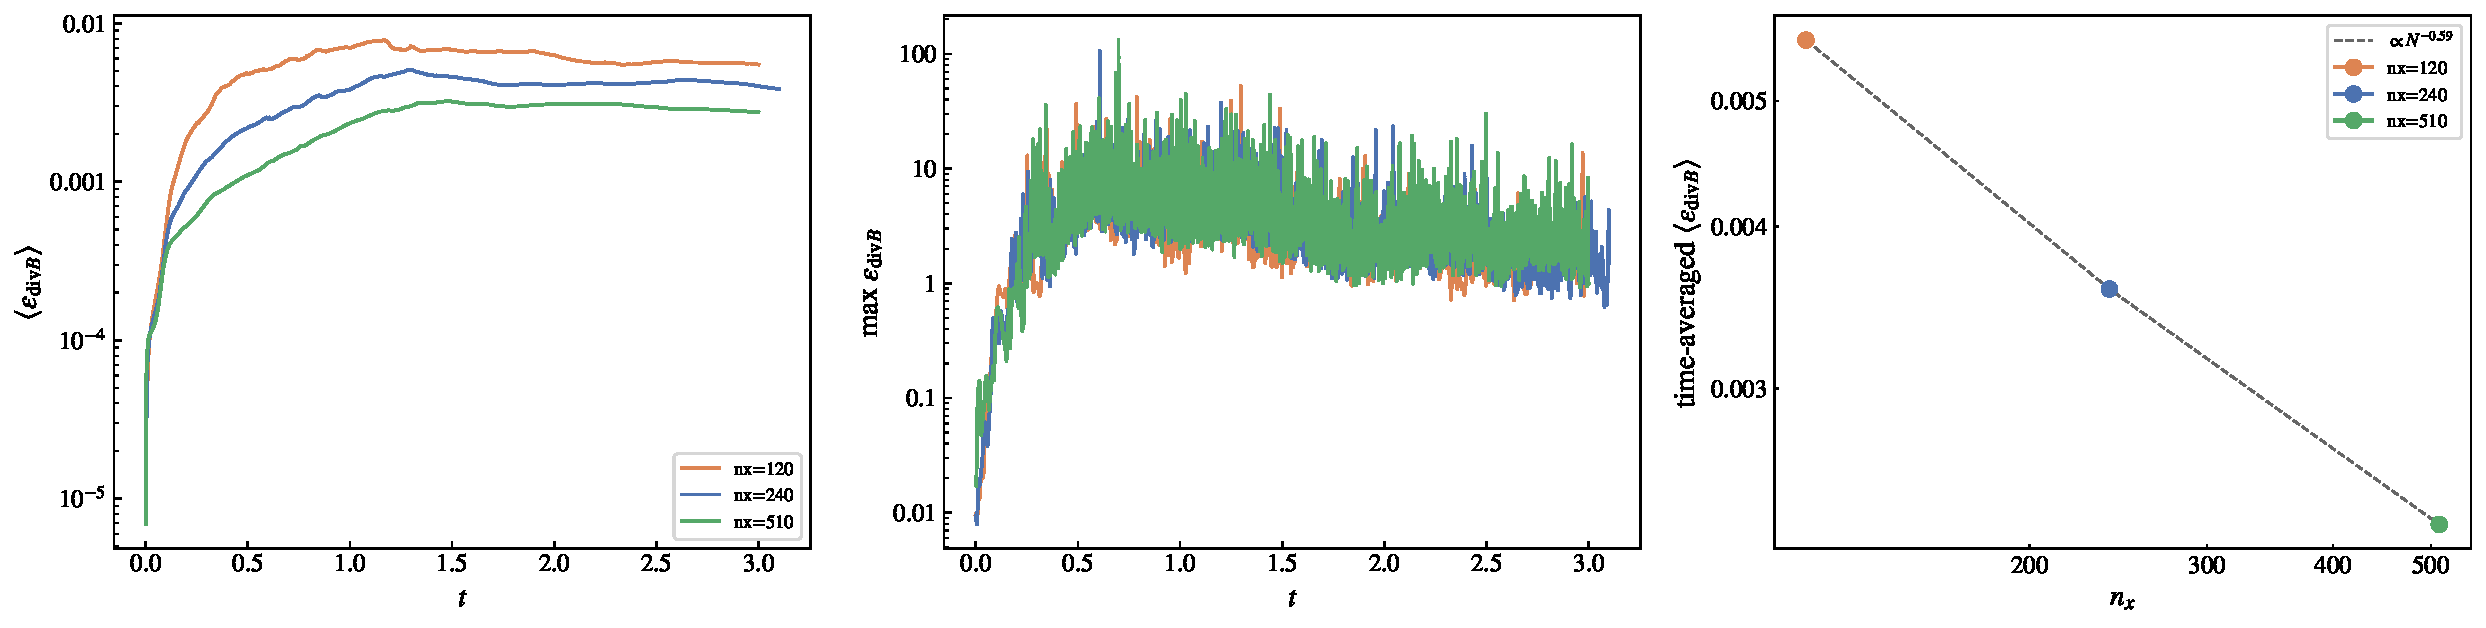
\includegraphics[width=\linewidth]{img/OT/compare_divb.pdf}
    \caption{Orszag-Tang vortex: Divergence error analysis. The first two panels show the mean divergence error $\langle\varepsilon_{\mathrm{div}B}\rangle$ and the maximum divergence error $\max (\varepsilon_{\mathrm{div}B})$ over time for three resolutions. In the last panel we see convergence of the time averaged mean divergence error with increasing resolution $n_x$.}
    \label{fig:ot_divb}
\end{figure}

% python sphexa/scripts/plot_constants_compare.py divb out/12686005_OT_120_t3/ out/12668681_OT_240_t3/ out/12685706_OT_510_t3/ --labels nx=120,nx=240,nx=510 --clean

% python sphexa/scripts/plot_slice.py out/9542508_OT_120/dump.h5 1 out/9542597_OT_240/dump.h5 1 out/9549515_OT_510/dump.h5 1 out/9542508_OT_120/dump.h5 2 out/9542597_OT_240/dump.h5 2 out/9549515_OT_510/dump.h5 2 --cmap gist_heat --labels nx=120 nx=240 nx=510 --label-time --clean --resolution 512

\subsection{MHD rotor}
\label{sec:rotor}

% Angular momentum handling. divB cleaning under strong twisting.
% anisotropically sampled (different from wissing)!! compresses the inner glass in xy only (halfA = L/sqrt(10), z multiplicity unchanged). simpler with glass blocks. rho=10 achieved. z-invariant test, therefore fine. just initial smoothing length distribution.

The MHD rotor of Balsara \& Spicer \cite{BalsaraSpicer1999} places a dense, rapidly rotating cylinder in a uniformly magnetized medium at rest. The rotor winds up the field and launches torsional Alfvén waves into the surrounding gas, which brake the cylinder and transport angular momentum outwards. For our purposes it is a robustness check to ensure that the divergence error and the resistive dissipation stay under control in a case dominated by rotation rather than shocks.

A periodic box of $L=[1,1,\frac{30}{n_x}]$ is initialized with an ambient medium of $\rho = 1$ at mean particle spacing $\Delta = 1/n_x$ with $n_x = 240$. The cylinder ($\rho = 10$, $R = 0.1$) is put into rotation, $v = (v_0/R)[-y, x, 0]$ with $v_0 = 2$, in a uniform field $B = [5/\sqrt{4\pi}, 0, 0]$ at uniform pressure $P = 1$ with $\gamma = 1.4$. The density contrast is unsmoothed, as in \cite{WissingShen2020}. We obtain it by compressing the glass block in $x$ and $y$ only (by $\sqrt{10}$, leaving the $z$ spacing untouched) rather than by a close-packed lattice. Since the test is $z$-invariant, this affects only the initial smoothing length distribution.

Figure \ref{fig:rotor} shows the magnetic pressure at $t=0.15$. The characteristic structure is reproduced: the tilted central lens of expelled field, the two magnetic pressure maxima above and below it, and the near-circular front of the outgoing wave. We choose the same limits $P_{mag} = [0, 2.642]$ as in \cite{Toth2000, Price2018, WissingShen2020}. The mean normalized divergence error is $\langle\varepsilon_{\mathrm{div}B}\rangle = 1.6 \times 10^{-3}$\todo{check divB number}. Repeating the run with the a05 scheme leaves the structure and the divergence error essentially unchanged ($1.8 \times 10^{-3}$) but dissipates $1.1\%$ of the initial magnetic energy through AR against $0.5\%$ for SLR.

\begin{figure}
    \centering
    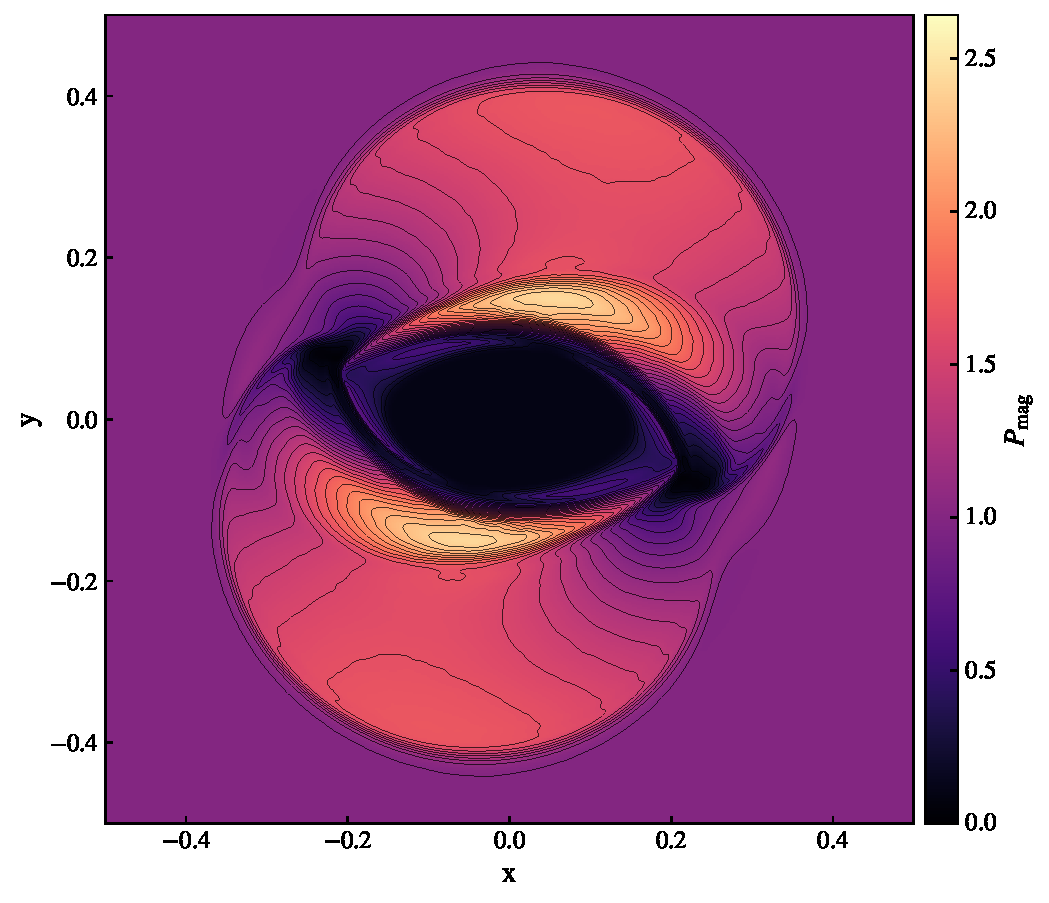
\includegraphics[width=0.7\linewidth]{img/Rotor/slice_Pmag_step1_z+0.0625_vmax2.642.pdf}
    \caption{MHD rotor magnetic pressure ($P_{mag} = B^2/2\mu_0$) at mid-plane ($z=0.0625$) and $t=0.15$ with $n_x = 240$, showing 30 contours using the same limits $P_{mag} = [0, 2.642]$ as in \cite{Toth2000, Price2018, WissingShen2020}.}
    \label{fig:rotor}
\end{figure}


\subsection{Magnetized Kelvin-Helmholtz instability}
\label{sec:kh}

% Instability physics: magnetic tension suppresses/reshapes KH roll-up. Verifies the code reproduces the field-strength-dependent growth-rate modification.
% t=1.6 hydro rolls look like the GDSPH panels, not TSPH. Thin arms, no blobbing, no visible surface-tension gaps at the interface. new VE scheme?
% Match growth rate to McNally.txt data. 

The Kelvin-Helmholtz (KH) instability grows at the interface of two fluids in shear flow and is the standard test for how well a code mixes across a contact discontinuity, a known weak point of traditional SPH. With a magnetic field applied parallel to the flow, magnetic tension acts against the deformation of the interface and slows the growth of the mode. %It is also the only test in this suite with a converged reference solution for a scalar growth measure.

We follow the setup of McNally et al. \cite{McNally2012} in the 3D form used in \cite{WissingShen2020}. A periodic box of $L= [1, 1, 0.0625]$ holds a dense inner stream $\rho_{in} = 2$ for $0.25 < y < 0.75$ and a light outer stream $\rho_{ext} = 1$, at uniform pressure $P = 5/2$. The inner stream moves at $v_{x,\mathrm{in}} = -0.5$ and the outer at $v_{x,\mathrm{out}} = +0.5$, joined by the exponential ramp of \cite{McNally2012} with smoothing scale $l_s = 0.025$, which makes the linear problem well-posed by removing the sharp velocity discontinuity. The instability is seeded by the single mode $v_y = 0.01 \sin(4 \pi x)$ and a uniform field $B = [-0.1, 0, 0]$ is applied along the flow. The dense stream is sampled at spacing $\Delta = 1/320$, i.e. $[n_x, n_y, n_z] = [320, 320, 20]$ over the full box, the light stream a factor $2^{1/3}$ coarser, giving $1.54 \times 10^6$ particles. We use $\texttt{ng0} = 100$ neighbors and run to $t = 3.2$. The same run was repeated with the magnetic field disabled.

McNally et al. also smooth over the \textit{density} jump in their (purely hydrodynamic) 2D problem. Wissing \& Shen \cite{WissingShen2020}, keep that jump sharp (in 3 out of 4 scenarios presented) so that it is smoothed only over the kernel and we adopt this. Note however that both our velocity and our magnetic field carry the opposite sign to theirs, making our configuration the mirror image in $x$. The physics is unchanged, but the rolls wind the other way. Also note that SPH-EXA does not implement artificial conductivity at this point in time.

Figure \ref{fig:kh_density} shows the density at $t = 1.6$, $2.6$ and $3.2$. Comparing to Fig. 9 in \cite{WissingShen2020} our results resemble their TSPH panels more closely than their GDSPH. The stretching of the vortex along the field reported in is visible in our panels as well, most clearly at $t=3.2$.

For a quantitative comparison we use the mode amplitude $M$. Figure \ref{fig:kh_growth} compares $M$ to the reference from \cite{McNally2012} on a logarithmic axis, where exponential growth in the linear phase appears as a straight line. Our hydrodynamic run tracks the reference closely, including the initial dip and the small oscillations before $t = 0.5$.% where an over-dissipative scheme would simply lose the seeded mode, and stays within $8\%$ (relative $L_1$) up to $t = 1.5$, ending about $10\%$ below it. We read this deficit as the numerical dissipation of our scheme at this resolution, consistent with the velocity noise floor discussed at the beginning of §\ref{sec:numerical_tests}. 
The magnetized run separates from it at $t \approx 0.7$, as soon as the interface deforms enough for magnetic tension to act, and reaches $22\%$ below the reference at $t = 1.5$. Saturation is earlier and weaker, $M_{max} = 0.16$ at $t \approx 2.0$ against $0.21$ at $t \approx 2.3$ without the field. Since the two runs are otherwise identical, the gap between them is due to the magnetic field alone.%, and at $B = 0.1$ the Alfvén speed stays well below the shear velocity, so the mode is slowed rather than suppressed.

\begin{figure}
    \centering
    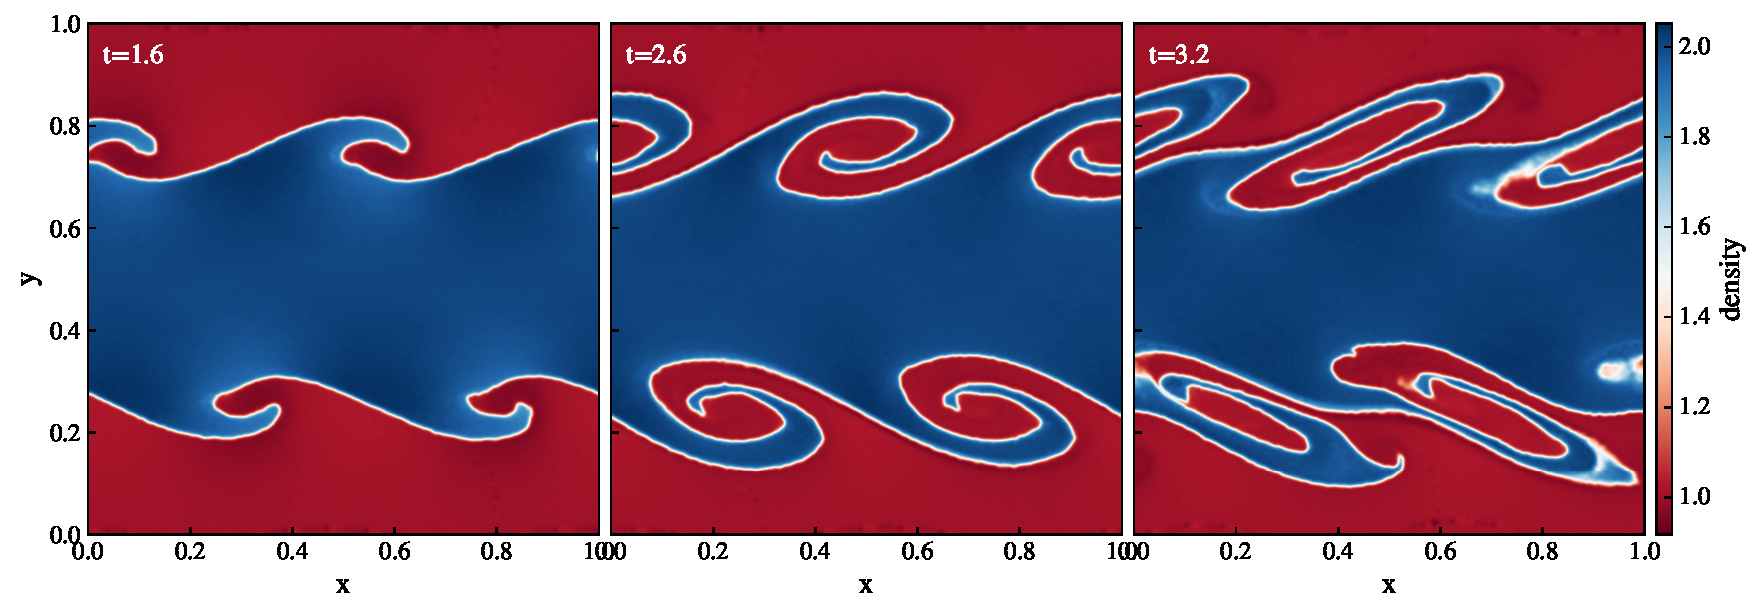
\includegraphics[width=\linewidth]{img/KH/slice_rho_step1_z+0.0312_panels.pdf}
    \caption{Magnetized Kelvin-Helmholtz instability: density slices in the mid-plane of the slab ($z = 0.031$) at $t=1.6$, $2.6$ and $3.2$, sampling the dense stream at $\Delta = 1/320$. To be compared with Fig. 9 in \cite{WissingShen2020}, noting that our configuration is mirrored in $x$ (see §\ref{sec:kh}).}
    \label{fig:kh_density}
\end{figure}

\begin{figure}
    \centering
    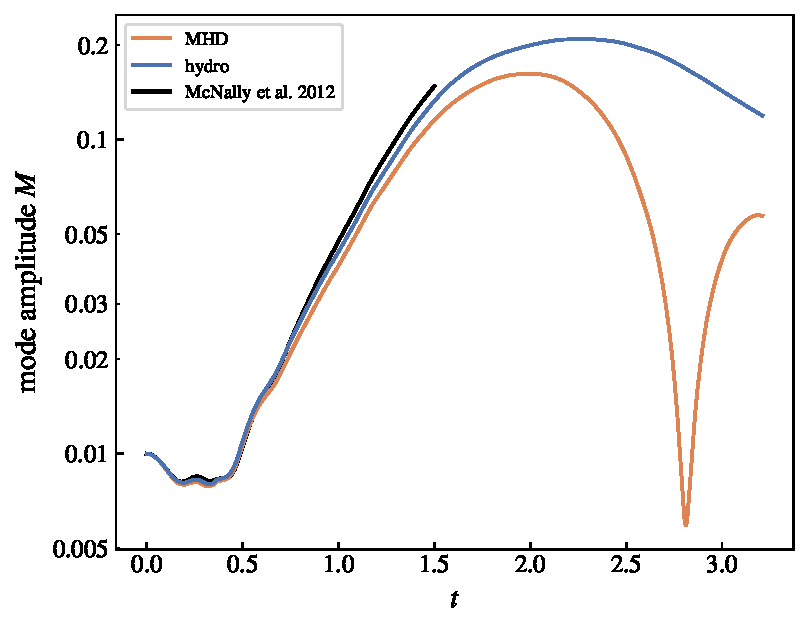
\includegraphics[width=0.5\linewidth]{img/KH/compare_kh.pdf}
    \caption{Kelvin-Helmholtz mode amplitude $M$ over time. The reference solution of McNally et al. \cite{McNally2012}, a converged 2D hydrodynamic grid result, is shown in black and ends at $t=1.5$. Our hydrodynamic run follows it closely, including the oscillations of the seeded mode before $t=0.5$. The magnetized run ($B = [-0.1,0,0]$) grows more slowly from $t \approx 0.7$ onwards and saturates earlier and at a lower amplitude, which is the expected effect of magnetic tension acting against the deformation of the interface.}
    \label{fig:kh_growth}
\end{figure}

% \begin{verbatim}
% python sphexa/scripts/plot_constants_compare.py kh out/12507482_KH_hydro_290c
%     out/12518185_KH_290c --labels hydro,MHD --clean --tmax 2.4
% \end{verbatim}

\subsection{Subsonic MHD turbulence}
\label{sec:mhd_turb}

After verifying our SPMHD implementation across seven standardized tests, we now want exploit the main advantage of SPH-EXA: its scalability on GPU clusters. The presented tests so far never exceeded more than a few million particles in resolution, 
%with the magnetized Sedov blast (§\ref{sec:sedov}) being the largest at $N=250^3\approx15.6M$ particles, 
keeping resolutions comparable to reference works. 

Here we model subsonic magnetic turbulence with $N=1600^3\approx4B$ particles. We use the pre-existing subsonic turbulence setup in SPH-EXA as presented in \cite{Cabezon2026} and simply extend it with a large-scale mean magnetic field. A periodic box of size $L=[1,1,1]$ is initialized with uniform density $\rho=1$, uniform pressure $P=1$ and a quasi-isothermal EOS with $\gamma=1.001$. The initially uniform magnetic field is set to $\mathbf{B_0}=[0,0.15,0]$. 

As in \cite{Cabezon2026}, turbulence is stirred by a stochastic Ornstein-Uhlenbeck forcing acting on wavenumbers $1 < |k| < 3$, with a parabolic amplitude distribution peaking at $k_c = 2$ and a mixture of $1/3$ compressive and $2/3$ solenoidal modes. 

The forcing amplitude targets an RMS velocity $v_\mathrm{rms} = 0.3$ which in this case corresponds to a sonic Mach number $\mathcal{M} \approx 0.3$ (in \cite{Cabezon2026} a statistically steady state is reached at $\mathcal{M} \sim 0.34$). The magnetic field strength defines the Alfvén speed $v_A = \mathbf{B}_0/\sqrt{\mu_0\rho} = 0.15$, giving a plasma beta $\beta = 2P/\mathbf{B}_0^2 \approx 90$ and an Alfvénic Mach number $\mathcal{M}_A = v_\mathrm{rms}/v_A \approx 2$. The setup is thus subsonic but mildly super-Alfvénic. 

Figure \ref{fig:turb} shows slices of the density, velocity field and magnetic field after $t=15$. Under magnetic tension the RMS Mach number only reaches $\mathcal{M}\sim0.19$, well below the $0.34$ of the purely hydrodynamic run. The mean divergence error $\langle \varepsilon_{\text{divB}}\rangle$ remains stable below $10^{-2.5}$.

\begin{figure}
    \centering
    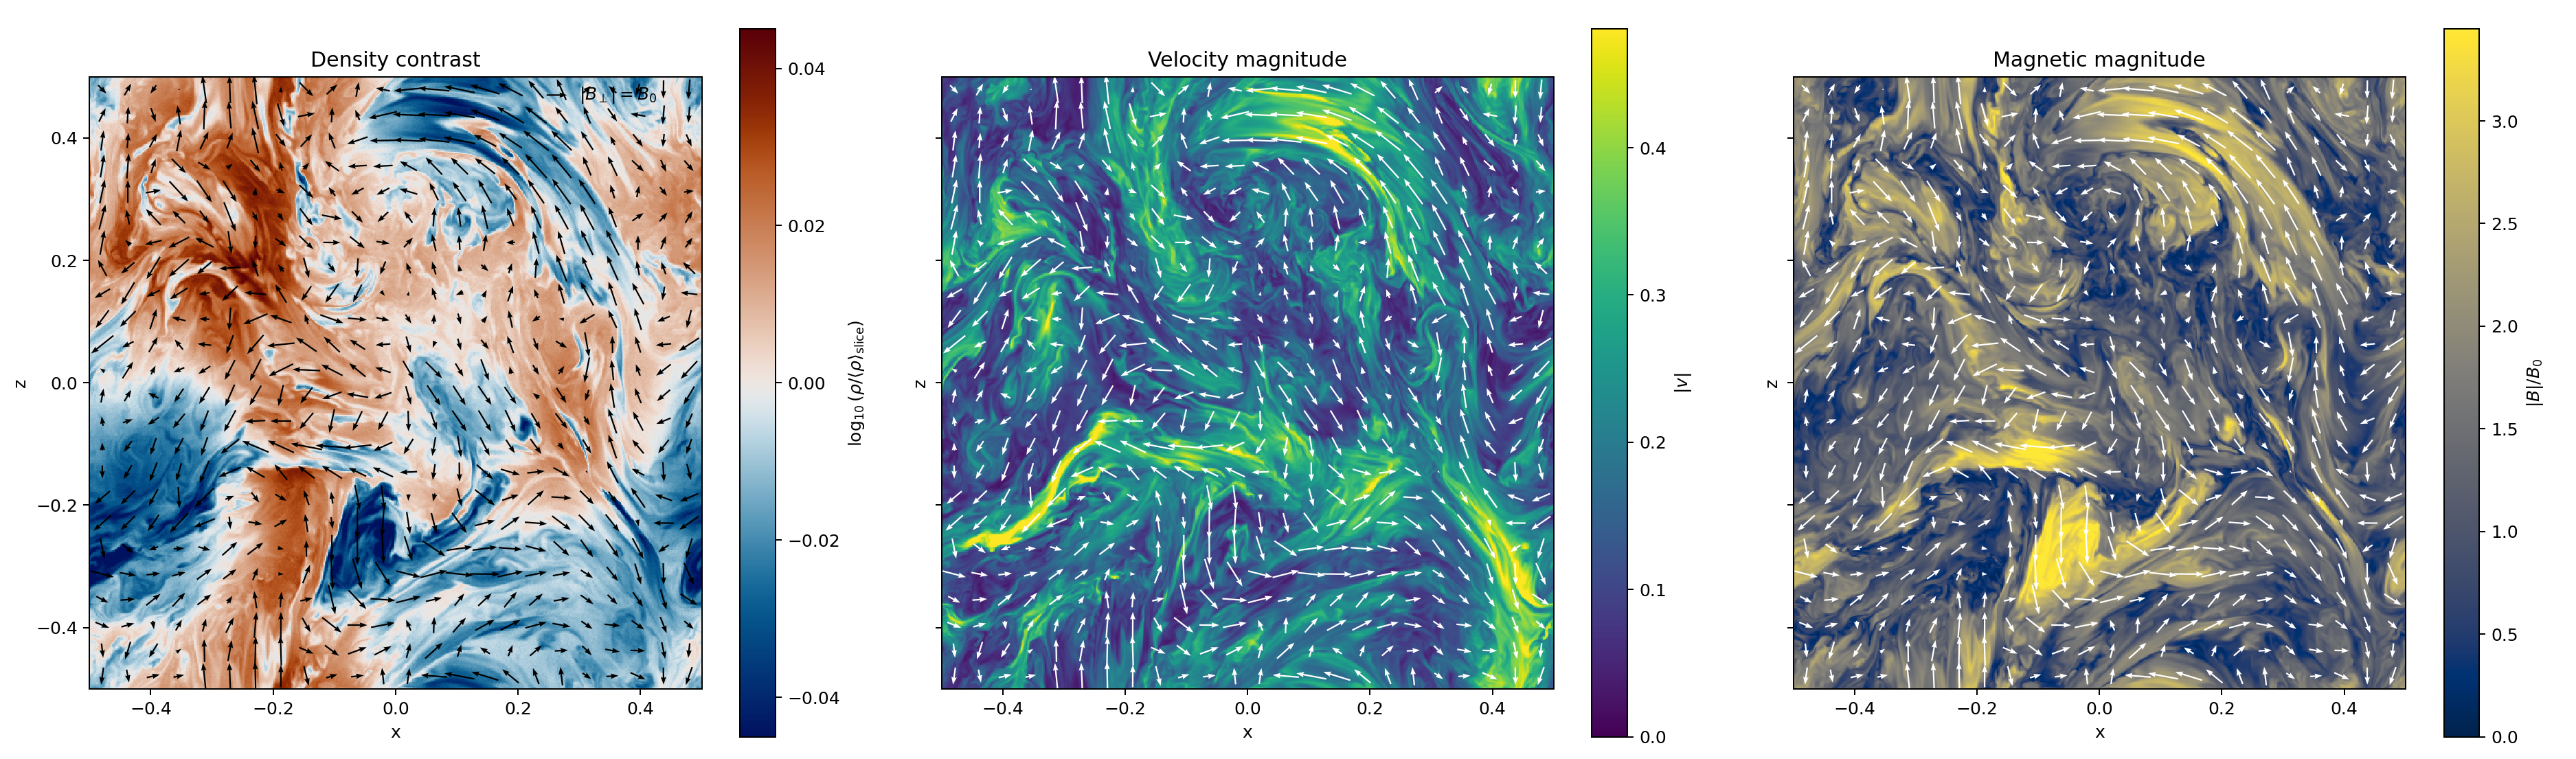
\includegraphics[width=\linewidth]{img/Turb/magnetic_slice_mpi_t15.0000_y+0.0000.png}
    \caption{Subsonic super-Alfvénic MHD Turbulence at $N=1600^3$ particles. Shown are thin slices (fixed size slab $y=0\pm 0.00125$) after $t=15$: Density contrast (\textit{left}), velocity magnitude (\textit{middle}) and normalized magnetic field magnitude (\textit{right}). Arrows show the magnetic field direction.}
    \label{fig:turb}
\end{figure}

% Timestep limit interesting. 
% Application. DivB error + resistive heating. $1600^3$ particles (more than 4 billion). 



\section{Discussion}
\label{sec:discussion}

In this Master Thesis, a complete implementation of ideal MHD in SPH-EXA was presented. The verification on standard MHD tests reproduces the reference results of \cite{WissingShen2020} and \cite{Price2018} accurately in structure and relevant metrics: the Alfvén wave reaches second-order convergence, the magnetized Sedov blast maintains energy conservation within $0.3\%$, the reference solution of the Brio-Wu shocktube is reproduced closely while keeping post-shock oscillations low, and the divergence error stays bounded and converges with increasing resolution across all tests. 

The MHD extension adds a computational overhead of $\sim 60\%$ wall time per iteration. Targeted optimization could likely reduce this further. In strong and weak scaling experiments the implementation matches the hydro baseline. The $1600^3$ turbulence simulation serves as a proof-of-concept that SPMHD in SPH-EXA is ready to tackle real astrophysical problems on Exascale computing systems. 

ARSLR achieved what we hoped for: small but distinct improvements over the `compromise' of a reduced resistivity coefficient on both fronts. In the shocktube test it does not under-dissipate, showing slightly less oscillation than the baseline, and in the noisy Alfvén wave it cleans uncorrelated noise more aggressively. At the same time it preserves the resolved structure of the Alfvén wave amplitude better and reduces resistive heating in all tests. It does so at reasonable computational cost of $4.8\%$ increased time per iteration. 

However, the improvements remain small and are not game-changing for the presented tests. In particular, no test in the suite exposes a case where the limiter fails, SLR under-dissipates, and the modulation of SLRB or SLRB2 would be needed. The parallel-component limiter is only partially motivated MHD and other limiter-designs, inspecting the transverse components separately, might still prove useful. It remains to be seen in which relevant scenarios ARSLR might bring real structural benefits and where it will fail. A well functioning and proven SLR scheme, which reliably protects resolved structure from unwanted dissipation, could potentially also open the door to further increase dissipation (e.g. by raising the coefficient $\alpha_B$ beyond 1) to hit real discontinuities harder without paying the price in other places. 

A recurring theme was that magnetic results are dominated by the choice of AV. Small-scale velocity noise leads to increased magnetic dissipation via the signal speed or enters the induction equation through the velocity gradient tensor. In the advection loop, the AV scheme ended up mattering far more than the AR scheme, with the most aggressive AV scheme leading to the best results. This suggests that smooth-flow MHD applications might benefit from a small constant floor of viscous dissipation being added. 

There is likely no optimal combination of AV and AR schemes that wins every race. A very recent paper \cite{Karapiperis2026} illustrates this: the authors implement SPMHD in \textsc{SWIFT} \cite{Schaller2024}, targeting cosmological simulations, and for that return to a variant of the Tricco \& Price switch combined with the Alfvén speed. They make the same diagnosis as us, finding the velocity-based signal speed to be overly dissipative in unconverged, disordered velocity fields. But the cures are different: they remove particle velocity from the signal speed; we remove the resolved part of $\mathbf{B}_{ab}$.

Until the holy grail is found, software should ideally offer users flexibility. 

%The search for better AR schemes is far from over. A very recent SPMHD implementation in \textsc{SWIFT} \cite{Karapiperis2026} illustrates this. Targeting cosmological simulations, the authors find the velocity-based signal speed of \cite{Price2018} to be overly dissipative in the unconverged, disordered velocity fields of coarsely resolved structures, and return to the Tricco \& Price steepness switch \eqref{eq:tp_switch}, combined with the Alfvén speed and a reduced $\alpha_\mathrm{max}$ following \cite{HopkinsRaives2016}. Their diagnosis is the one made in §\ref{sec:ar} and confirmed by the advection loop in §\ref{sec:MHD_loop}: $v_{\mathrm{sig},B}$ is purely kinematic and any unresolved velocity structure switches it on. The cures are complementary. They remove the velocity from the signal speed; we remove the resolved part of $\mathbf{B}_{ab}$, which is what lets ARSLR preserve the mode of the noisy Alfvén wave while removing the noise, something a per-particle scalar cannot do. Where both the field and the velocity are unresolved, ARSLR dissipates at full strength and their objection applies to it as well; we have not tested that regime. The SLRB variants already carry the Tricco \& Price measure as a modulator, so combining reconstruction with an Alfvén-speed signal velocity is a one-line change in SPH-EXA and the natural next experiment.

%The search for better AR schemes is far from over. A very recent SPMHD implementation in \textsc{SWIFT} \cite{Karapiperis2026} illustrates this: targeting cosmological simulations, the authors find the velocity-based signal speed of \cite{Price2018} to be overly dissipative in unconverged, disordered velocity fields, and return to the Tricco \& Price steepness switch \eqref{eq:tp_switch} combined with the Alfvén speed, following \cite{HopkinsRaives2016}. 

%the authors find the velocity-based signal speed of \cite{Price2018} to be overly dissipative in the unconverged, disordered velocity fields of coarsely resolved cosmological structures, and return to the Tricco \& Price steepness switc

%Their diagnosis is the same as ours in §\ref{sec:ar}: $v_{\mathrm{sig},B}$ is purely kinematic and fires on velocity noise. They remove the velocity from the signal speed; we remove the resolved part of $\mathbf{B}_{ab}$. Which approach is preferable likely depends on the application, and combining them is an obvious next step.

% AV and AR closely linked. Cannot separate.
% (Iwasaki & Inutsuka 2011) Riemann solvers? increased cost. 
% That new paper using switches again. 
% Outlook on better limiter, constructed with separate aggregation
% optimization work? 

% \paragraph{No single best configuration.}
% There is no combination of AV and AR schemes that wins in every test. The practical conclusion is that the code should offer the options and that the user must know the problem being simulated. 

% \paragraph{Outlook.}
%\todo{cite the recent paper returning to switches and position SLR relative to it} 
% Beyond dissipation, the natural extensions are non-ideal MHD terms and a kernel and initial-condition setup that preserves lattices, which would remove the noise floor that currently limits several tests.

\newpage
\bibliographystyle{unsrt}  
\bibliography{references}  


\end{document}
